\renewcommand{\d}{\mathrm{d}}


\chapter{Diskrete Mannigfaltigkeiten}

\section{Primär- und Dualgitter}
  
  \begin{ziel}
    Bei vielen numerischen Methoden werden Gebiete, über nichtabzählbaren Mengen auf denen Gleichungen "`leben"', diskretisiert.
    Ziel dabei ist es, endlich viele Gleichungen zu erzeugen, die das ursprüngliche Problem approximativ lösen.
    Ein Beispiel für solch ein Vorgehen ist die FDM (Finite-Differenzen-Methode) im \( \R^{n} \).
    Dort wird ein Gebiet \( U\subseteq\R^{n} \) mit endlich vielen Rechtecken diskretisiert 
    und es wird versucht eine Funktion zu finden, die jedem Knoten einen Wert zuweist und damit endlichdimensional beschrieben ist, sodass diese
    diskrete Funktion eine stetige Funktion auf \( U \) approximiert. 

    Das funktioniert beim DEC ähnlich. Die Objekte, die es hier zu approximieren gilt, sind allerdings Differentialformen und das Gebiet eine
    Mannigfaltigkeit, welche durch Polyeder diskretisiert wird. Die diskreten Differentialformen werden dann auf den Knoten, Kanten, Flächen usw. als Integralwerte
    definiert. Wir werden uns hierbei auf Simplizes als spezielle Polyeder beschränken und die Menge der Simplizes so charakterisieren, dass wir
    eine algebraische Topologie bekommen. Somit wird eine algebraische Struktur erzeugt, die es einem ermöglicht in dieser Topologie
    "`sinnvoll zu rechnen"'.
    Das heißt der große Unterschied zu anderen numerischen Verfahren ist, dass wir nicht auf einem Gitter sondern mit einem Gitter rechnen wollen.
    Aus diesem Grund müssen Anforderungen an die diskrete Struktur gestellt werden, welche bestimmte Eigenschaften der Differentialformen auch widerspiegeln.
    So bilden die Differentialformen auf einer Mannigfaltigkeit zusammen mit der äußeren Ableitung einen Kokettenkomplex, den de-Rham-Kokomplex, und mit ihm die de-Rham-Kohomologiegruppen.
    Kohomologiegruppen lassen sich mit Hilfe eines Rand\-operators auch erzeugen, deshalb scheinen zum
    Beispiel
    die Simplizialkomplexe, als Triangulierung einer Mannigfaltigkeit, ein geeigneter Kandidat für
    eine Gitterstruktur zu sein.
    Wie wir später noch in Kapitel \ref{chapterDEC} sehen werden, haben wir mit der de-Rham-Abbildung eine Möglichkeit mit der sich Elemente aus dem de-Rham-Kokomplex
    (Differentialformen) auf dem simplizialen Kokettenkomplex (diskrete Differentialformen) identifizieren lassen.
    Dazu sind aber einige Voraussetzungen an das Gitter nötig, die im Folgenden eingeführt werden.
    Zudem wird in Abschnitt \ref{secGittergenerierung} eine einfache Möglichkeit geboten, bestehende Gitter an diese Anforderungen anzupassen.
  \end{ziel}

  \subsection{Simplizialkomplex}
    
    Die Elemente des noch zu definierenden Simplizialkomplexes sind die Simplizes.
    Diese wollen wir hier erst einmal geometrisch als Teilmenge des \( \R^{N} \) einführen.

    \begin{definition}
      \label{defSimplex}
      Ein \( p \)-Simplex ist die konvexe Hülle von \( p+1 \) geometrisch unabhängigen Punkten im \( \R^{N} \), d.h.
      \begin{align}
        \sigma^{p} &:= \left\{  x \in \R^{N} \middle| x = \sum_{i=0}^{p}\mu^{i}v_{i} \text{ wobei } \mu^{i} \ge 0  \text{ und } \sum_{i=0}^{p}\mu^{i} = 1 \right\}
      \end{align}
    \end{definition}
    
    Geometrisch unabhängig bedeutet dabei, dass die \( p \) Vektoren \( v_{1} - v_{0}, v_{2} - v_{0},\ldots,  v_{p} - v_{0} \) linear unabhängig sind.
    Konkret werden wir je nach Kontext \( \sigma^{0} \) Knoten, Ecke oder Gitterpunkt, \( \sigma^{1} \) Kante und \( \sigma^{2} \) Dreieck(element) oder Volumenelement nennen.
    Des Weiteren schreiben wir auch kurz \( \sigma^{p} = v_{0} v_{1} \ldots v_{p} \) und sagen 
    "`Das Simplex \( \sigma^{p} \) wird von den Ecken \( \{ v_{0}, v_{1}, \ldots, v_{p}\} \) aufgespannt."'.

    \begin{bemerkung}
      \label{singSimplex}
      \label{refSingSimplex}
      Die obige Definition eines Simplexes, hier als \( \sigma_{\text{geo}} \) geschrieben, nennt man auch geometrische Realisierung eines Simplexes.
      Denn es ist auch möglich, ein Simplex als Abbildung vom Standard-Simplex 
        \begin{align} 
          \Delta^{p} &:= \left\{\left( \mu^{0},\mu^{1},\ldots,\mu^{p} \right) \middle| \mu^{i} \ge 0  \text{ und } \sum_{i=0}^{p}\mu^{i} = 1 \right\} \subset
        \R^{p+1} 
        \end{align}
      in einen Topologischen Raum zu definieren, im obigen Fall in den \( \R^{N} \). 
      Mit Hilfe der Ecken \( v_{i}\in\R^{N} \) können wir die Abbildung festlegen durch
      \begin{align}
        \sigma_{\text{sing}} = \sigma^{p}_{\text{sing}}\left( v_{0}, v_{1}, \ldots, v_{p} \right) : \Delta^{p} &\rightarrow \R^{N}
                        : \left( \mu^{0},\mu^{1},\ldots,\mu^{p} \right)\mapsto \sum_{i=0}^{p}\mu^{i}v_{i}
      \end{align}
      sodass \( \sigma_{\text{sing}}(\Delta^{p}) = \sigma^{p}_{\text{geo}} \) gilt.
      Das Simplex \(\sigma_{\text{sing}}\) heißt singuläres \( p \)-Simplex (vgl. \cite{lueck}).
    \end{bemerkung}

    Von nun an ist mit einem Simplex \( \sigma \) immer die geometrische Realisierung nach Definition \ref{defSimplex} gemeint, solange nicht explizit auf
    etwas anderes hingewiesen wird.
    
    Eine Größe, die wir noch häufig benötigen werden, ist das Volumen eines Simplexes.
    \begin{definition}
      Das Volumen eines \( p \)-Simplexes \( \sigma^{p} \) für \( p > 0 \) ist definiert durch
      \begin{align}
        \left| \sigma^{p} \right| &:= \int_{\sigma^{p}} dx^{1}\wedge dx^{2} \wedge \ldots \wedge dx^{p}\formkomma
      \end{align}
      wobei \( \left( x^{1}, x^{2}, \ldots, x^{p} \right) \) die Koordinaten des \( p \)"~Dimensionalen Untervektorraumes des
      \( \R^{N} \) sind in dem \( \sigma^{p} \) liegt.
      Für \( p=0  \) definieren wir
      \begin{align}
        \left| \sigma^{0} \right| &:= 1 \formpunkt
      \end{align}
    \end{definition}
    Damit ist das Volumen einer Ecke gleich null, von einer Kante die Länge und von einem Dreieck der Flächeninhalt.


    \begin{definition}
      Für \( 0 \le r < p \) definiert sich eine Relation zwischen dem \( r- \)Simplex \(\sigma^{r}\) und dem \( p- \)Simplex \( \sigma^{p}:= v_{0} v_{1} \ldots v_{p} \) durch
      \begin{align}
        \sigma^{r} \prec \sigma^{p} &:\Leftrightarrow \sigma^{p} \succ \sigma^{r} \\
                                    &:\Leftrightarrow \exists \{ v_{i_{0}}, v_{i_{1}}, \ldots, v_{i_{r}} \} \subset \{ v_{0}, v_{1}, \ldots, v_{p}\} : \sigma^{r} = v_{i_{0}} v_{i_{1}} \ldots v_{i_{r}}
      \end{align}
      und \( \sigma^{r} \) nennen wir Facette oder Seite von \( \sigma^{p} \).
    \end{definition}
    
    Damit bildet \( \prec \) bzw. \( \succ \) eine strikte Ordnung auf der Menge aller (endlichen) Simplizes.
    
    \begin{definition}
      Ein Simplizialkomplex \( K \) über \( \R^{N} \) ist eine Menge von Simplizes mit folgenden zwei Regeln
      \begin{itemize}
        \item Jede Facette eines Simplexes aus \( K \) ist ebenfalls aus \( K \).
        \item Der Schnitt zweier Simplizes aus \( K \) ist entweder eine Facette von beiden oder leer.
      \end{itemize}
      Dabei heißt
      \begin{align}
        n &:= \text{dim}(K) := \max\left\{ p \in \mathds{N} \middle| \sigma^{p} \in K \right\}
      \end{align}
      die Dimension von \( K \) und \( N \) bezeichnet die Dimension des Ambienteraumes, in unserem Fall also des \( \R^{N} \).
    \end{definition}

    Im Folgenden ist ein Simplizialkomplex immer endlich. Das heißt, er besteht nur aus einer endlichen Menge von Simplizes.

    \begin{definition}
      Die Vereinigung aller Simplizes eines Simplizialkomplexes über \( \R^{N} \), das heißt
      \begin{align}
        |K| := \bigcup_{\sigma \in K} \sigma \subset \R^{N} \text{,}
      \end{align}
      ist der zugrunde liegende (topologische) Raum oder auch Polytop.
      Die Topologie von \( |K| \) ist dann gerade die induzierte Teilraumtopologie des \( \R^{N} \).
    \end{definition}
    
    In den meisten Fällen wird jedoch ein Raum gegeben sein und es ist ein entsprechender Simplizialkomplex gesucht, der diesen Raum beschreibt.
    Dieses führt uns zu folgender Definition.

    \begin{definition}
      Ein Simplizialkomplex \( L \) heißt (simpliziale) Triangulation von \( V \subset \R^{N} \), wenn \( |L| = V \) gilt.
      Existiert eine Triangulation von \( V \), dann heißt \( V \) triangulierbar.
    \end{definition}

    Bisher kann solch ein Simplizialkomplex noch sehr viele Teilräume des \( \R^{N} \) beschreiben, welche für diese Arbeit nicht von Belang sind. 
    Wir wollen deshalb die Menge der Simplizialkomplexe etwas einschränken, um uns langsam der Beschreibung von 
    \mbox{(Hyper-)Oberflächen} zu nähern.

    \begin{definition}
      Ein Simplizialkomplex \( K \) heißt mannigfaltigartig, wenn das Polytop \( |K| \) eine \( C^{0} \)-Mannigfaltigkeit ist.
    \end{definition}

    Da wir uns später mit dem Spezialfall von Oberflächen im \( \R^{3} \) beschäftigen möchten, seien hier schon mal ein paar Bemerkungen dazu.
    
    \begin{bemerkung}
      Sei \( K \) ein zweidimensionaler mannigfaltigartiger Simplizialkomplex im \( \R^{3} \).
      \begin{itemize}
        \item Falls \( |K| \) nicht flach ist, dann ist das Polytop \( |K| \) global nicht differenzierbar.
        \item Falls \( |K| \) zudem eine geschlossene Mannigfaltigkeit ist, dann ist \( |K| \) ein Polyeder.
      \end{itemize}
    \end{bemerkung}

    Der zugrunde liegende Raum eines Simplizialkomplexes kann im Allgemeinen nicht eine beliebige 
    \( C^{\infty} \)-Mannigfaltigkeit sein. Jedoch kann ein Simplizialkomplex solch eine
    Mannigfaltigkeit approximieren, d.h.
    
    \begin{definition}
      \label{defManniApprox}
      Ist \( K \) ein man\-nigfaltigartiger Simplizialkomplex und \( M \) eine \( C^{\infty} \)"~Man\-nigfaltigkeit, dann sei
      \begin{align}
        K \sim M &:\Leftrightarrow \forall \sigma^{0}\in K : \sigma^{0} \in M \formpunkt
      \end{align}
      Das heißt \( K \) approximiert \( M \) genau dann, wenn alle Ecken von \( K \) auch auf \( M \) liegen.
    \end{definition}

    \begin{bemerkung}
      Wenn \( K \sim M \) gilt, dann würden wir für die Übertragung von skalarwertigen Informationen von der Mannigfaltigkeit
      \( M \) auf den Simplizialkomplex \( K \) auf den Ecken nichts falsch machen.
      Wie sieht es aber mit höherwertigen Informationen, wie zum Beispiel Vektorfelder oder 
      allgemein Differentialformen höheren Grades als null, aus?
      Für zweidimensionale Mannigfaltigkeiten bedeutet dies, dass 1-Formen auf Kanten und 2-Formen auf den Dreieckelementen ausgewertet
      werden. Wie wir später noch in Kapitel~\ref{chapterDEC} sehen werden.
      Kanten und Dreieckflächen liegen aber nur (linear) approximiert im Simplizialkomplex vor, genauso wie auch die Metrik,
      da die Simplizes im Inneren flach sind.
      Dennoch brauchen wir für spätere Argumentationen ein simpliziales Konstrukt, bei dem wir diese Fehler nicht machen.
      Diese formale Brücke zwischen der Mannigfaltigkeit und dem Simplizialkomplex nennen wir abstrakter Simplizialkomplex (über der Mannigfaltigkeit \( M \) ). 
      Er lässt sich genauso einführen wie oben für den Simplizialkomplex über dem \( \R^{N} \), 
      nur dass die \(p\)-Simplizes für \( p > 0 \) eine Krümmung besitzen. Und zwar ist es die gleiche wie für \( M \) eingeschränkt auf das jeweilige Simplex.
      Das heißt, dass der zu grundeliegende Raum des abstrakten Simplexes gleich der Mannigfaltig \( M \) ist.
      Folgendes kommutative Diagramm, soll das für ein einzelnes Simplex verdeutlichen.
      \begin{align}
        \label{diagSingulaerAbstrakt}
        \begin{xy}
          \xymatrix{
            **[l] \R^{p+1} \supset \Delta^{p} \ar[rr]^{\sigma_{\text{sing}}} \ar[rd]_{\hat{\sigma}_{\text{sing}}} 
            & & **[r] \sigma^{p} \subset \R^{N} \ar[ld]_{\pi_{\sigma}} \\
                                       & **[r] \sigma^{p}_{M}\subset M&
          }
        \end{xy}
      \end{align}
      Die Abbildungen \( \sigma_{\text{sing}} \) und \( \hat{\sigma}_{\text{sing}} \) sind singuläre Simplexe, wie in
      Bemerkung \ref{singSimplex} definiert. \( \sigma^{p} \) und \( \sigma^{p}_{M} \) sind deren geometrische Realisierungen im \( \R^{N} \) beziehungsweise auf \( M \)
      und es gelte \( \sigma^{p} \sim \sigma^{p}_{M} \).
      \( \pi_{\sigma} \) ist ein Homöomorphismus, das heißt bijektiv, stetig und \( \pi_{\sigma}^{-1} \) ist ebenfalls stetig.
      Whitney \cite{whitney} forderte noch weitere Bedingungen an diese Abbildung. 
      Für uns soll die Homöomorphieeigenschaft allerdings reichen, da wir sie nur formal nutzen werden und nie explizit mit ihr rechnen wollen.
      Prinzipiell genügt es, wenn wir uns die Abbildung \( \pi_{\sigma} \) als "`Ankleben"' des Simplexes \( \sigma \) auf die Mannigfaltigkeit vorstellen.
      Des Weiteren soll \( \pi:=\pi_{\bullet} \) \footnote{d.h. \( \pi|_{\sigma} = \pi_{\sigma} \)} homomorph auf dem ganzen Simplizialkomplex bezüglich der Relation \( \prec \) sein, 
      also ist \( \pi \) ein Isomorphismus zwischen dem Simplizialkomplex \( K \) und einem abstrakten Simplizialkomplex \( L \) mit \( |L| = M \) und \( K^{(0)} = L^{(0)} \).
      Wobei
      \begin{align}
        K^{(p)} &:= \left\{ \sigma^{p} \in K \right\}
      \end{align}
      das \( p \)-Skelett von \( K \) ist. 
      Zudem ist \( L = \pi(K) \) somit eindeutig bestimmt, falls \( \pi \) bekannt ist.
      Wenn solch eine Triangulation \( L \) von \( M \) existiert, dann nennen wir auch \( K = \pi^{-1}(L) \) eine (lineare) Triangulation von \( M \).
    \end{bemerkung}

    Später werden wir häufig den Begriff "`1-Ring"' verwenden.
    Meistens sind damit die Menge der Dreieckelemente gemeint, die eine gemeinsame Ecke besitzen, 
    im Falle einer triangulierten Oberfläche.
    Dieser Begriff lässt sich auch allgemeiner fassen.
    \begin{definition}
      Es sei \( K \) ein \( n \)-dimensionaler mannigfaltigartiger Simplizialkomplex,
      dann bezeichnet die Menge
      \begin{align}
        \left\{ \sigma^{n}\in K \middle| \sigma^{p}\prec\sigma^{n} \right\} & \subseteq K^{(n)}
      \end{align}
      den 1-Ring um \( \sigma^{p}\in K \).
    \end{definition}

    Für den DEC ist der Begriff der Orientierung von essenzieller Bedeutung. 
    Zum einen weil die Orientierung der Simplizes über das Vorzeichen eines Berechnungsschemata entscheiden kann 
    und zum anderen wird eine weitere notwendige Eigenschaft an den Simplizialkomplex, dessen Polytop und die zu 
    approximierende Mannigfaltigkeit gestellt: die Orientierbarkeit.

    Wie wir in Bemerkung \ref{refSingSimplex} sehen, hängt die geometrische Realisierung \( \sigma \) eines singulären Simplexes \( \sigma_{\text{sing}} \), 
    also dessen Bild, nicht von der gewählten Reihenfolge der Ecken \( v_{i} \) ab. 
    Formal können wir aber diesen für \( \sigma \) syntaktischen Unterschied auch semantisch nutzen und schreiben \( \sigma = \left( v_{0}, v_{1}, \ldots, v_{p} \right) \)
    mit runden Klammern, um die Reihenfolge zu würdigen. 
    Somit ergeben sich für einen Satz Ecken \( p! \) Simplizes 
    \begin{align}
      \Sigma^{p} &:= \left\{ \left( v_{\tau(0)}, v_{\tau(1)}, \ldots, v_{\tau(p)} \right) \middle| \tau\in S_{p} \text{ Permutation} \right\} \formkomma
    \end{align}
    die geometrisch das gleiche Simplex beschreiben.
    Auf \( \Sigma^{p} \) lässt sich nun eine Äquivalenz\-re\-la\-tion \( \Theta \subseteq \Sigma^{p}\times\Sigma^{p} \) definieren:

    \begin{definition}
      \label{defAeqRel}
      Es sei \( \sigma_{1} = \tau(\sigma_{2})\in\Sigma^{p} \), dann gelte
      \begin{align}
        \sigma_{1} \Theta \sigma_{2} &:\Leftrightarrow \tau \in A_{n} \text{ gerade Permutation,}
      \end{align}
      wobei \( \tau(\sigma) := \left( v_{\tau(0)}, v_{\tau(1)}, \ldots, v_{\tau(p)} \right) \) 
      für \( \sigma = \left( v_{0}, v_{1}, \ldots, v_{p} \right) \) ist.
      Ein Element des Faktorraumes \( \Sigma^{p}\slash\Theta \) heißt orientiertes Simplex und wir schreiben dafür
      \begin{align}
        \sigma &= \left[ v_{0}, v_{1}, \ldots, v_{p} \right]
      \end{align}
    \end{definition}

    Dass hier das orientierte Simplex ebenfalls als \( \sigma \) geschrieben wird soll, uns nicht stören, da dieses auch immer das entsprechende geometrische Simplex impliziert.
    Oft werden wir einfachheitshalber nur Simplex sagen, wenn aus dem Kontext klar ist, dass dieses Simplex orientiert ist.
    Für \( p > 0 \) ergeben sich somit genau 2 Äquivalenzklassen und somit Orientierungen pro Simplex. 
    Wir wollen die Orientierung eineindeutig mit 
    \begin{align}
      \sgn: \Sigma^{p}\slash\Theta \rightarrow \left\{ -1 , +1 \right\}
    \end{align}
    beschreiben.
    Falls \( p=0 \), das heißt es liegt eine Ecke vor und folglich nur eine Orientierungsmöglichkeit, dann wird die Orientierung festgelegt. 
    Wenn möglich durch die induzierte Orientierung.

    \begin{definition}
      \label{defIndOri}
      Es sei \( \sigma^{p} = \left[ v_{0}, v_{1}, \ldots, v_{p} \right] \in \Sigma^{p}\slash\Theta \) mit \( p \ge 1 \), 
      dann definiert sich eine induzierte Orientierung für die \( (p-1) \)-Facetten von \( \sigma^{p} \) durch
      \begin{align}
        \sgn\left( \left[ v_{0}, v_{1}, \ldots, \hat{v_{i}}, \ldots, v_{p} \right] \right) &:=
        \begin{cases}
          \sgn(\sigma^{p}) & \text{falls } i \text{ gerade,} \\
          -\sgn(\sigma^{p}) & \text{falls } i \text{ ungerade,} 
        \end{cases}
      \end{align}
      wobei \( \left[ v_{0}, v_{1}, \ldots, \hat{v_{i}}, \ldots, v_{p} \right] \) bedeutet, dass die \( i \)-te Ecke weggelassen wird.
    \end{definition}

    \begin{beispiel}
      \label{bspOrientierung}
      Anhand folgendem Beispieles sehen wir, dass diese Definition intuitiver ist als es vielleicht auf den ersten Blick anmuten mag.
      Gegeben sei ein \( 2 \)-Simplex \mbox{\( \sigma:=\left[ v_{0}, v_{1}, v_{2} \right] \)}, also ein Dreieck, dessen Orientierung auf \( +1 \) festgelegt wird.
      Daraus leiten sich die Orientierungen der Kanten ab. 
      Durch Transposition der Kante \( \left[ v_{0}, v_{2} \right] \), und damit dem Wechsel zur anderen Äquivalenzklasse, 
      kann zudem eine einheitliche Orientierung aller Kanten erreicht werden.
      \begin{align}
        \begin{xy}
          \xymatrix{
            & \sgn\left( \left[ v_{0}, v_{1}, v_{2} \right] \right):=+1 \ar@{=>}[ld] \ar@{=>}[d] \ar@{=>}[rd]& \\
            \sgn\left( \left[ v_{0}, v_{1} \right] \right)=+1 &
            \sgn\left( \left[ v_{0}, v_{2} \right] \right)=-1 \ar@{=>}[d] &
            \sgn\left( \left[ v_{1}, v_{2} \right] \right)=+1 \\
            & \sgn\left( \left[ v_{2}, v_{0} \right] \right)=+1 &
          }
        \end{xy}
      \end{align}
      \begin{minipage}{0.65\textwidth}
        Geometrisch wird die Orientierung oft durch Pfeile visualisiert.
        In diesem Beispiel ist es ein gebogener Pfeil für die Fläche.
        Gegen den Uhrzeigersinn bedeutet hierbei eine Orientierung von \( +1 \). 
        Dies ist auch gleichbedeutend damit, 
        dass die Rechte-Hand-Regel 
        gilt und die Fläche per Definition eine äußere Normale besitzt.
        Sollen nun alle Kanten die gleiche Orientierung wie die Fläche besitzen, so müssen die Pfeile der Kanten ebenfalls gegen den Uhrzeiger abgetragen werden.
        Von nun an werden wir Pfeile ohne Beschriftung immer als positiv, also mit Orientierung \( +1 \), anerkennen.
      \end{minipage}
      \hfill
      \begin{minipage}{0.3\textwidth}  
      \begin{tikzpicture}[>=latex]
        % Coords
        \coordinate (V0) at (0,0);
        \coordinate (V1) at (2,0);
        \coordinate (V2) at (1,2);
        % Arrows\tilde{\sigma}
        \draw[line width=1pt, ->]
          (V0) -- node[below] {\( +1 \)} (V1);
        \draw[line width=1pt, ->]
          (V1) -- node[above right] {\( +1 \)} (V2);
        \draw[line width=1pt, ->]
          (V2) -- node[above left] {\( +1 \)} (V0);
        % Points
        \fill (V0) node[below left] {\( v_{0} \)} circle (2pt);
        \fill (V1) node[below right] {\( v_{1} \)} circle (2pt);
        \fill (V2) node[above] {\( v_{2} \)} circle (2pt);
        % circ arrow
        \coordinate (C) at (1,0.666);
        \node at (C) {\( +1 \)};
        \def\r{0.35} 
        \draw[line width=1pt, ->] ($(C)+(135:\r)$) arc (135:405:\r) -- ++ (-3pt,3pt);
      \end{tikzpicture}
      \end{minipage}\\
      \vspace{0.5cm}\\
      \noindent\begin{minipage}{0.65\textwidth}
      \noindent Es sei nun ein weiteres Simplex \( \tilde{\sigma} := \left[ v_{1}, v_{3}, v_{2} \right] \) "`angelegt"', sodass beide Simplizes sich die Kante
      \( \left[ v_{1}, v_{2} \right] \) teilen und die Orientierung von \( \tilde{\sigma} \) auf \( +1 \) gesetzt wird. 
      Dabei müssen die von den Kanten aufgespannten (Unter"~)Vektorräume (z.B. des \( \R^{3} \)) nicht notwendigerweise gleich sein.
      Dennoch liegt das Gefühl nahe, zu sagen, dass die beiden 2-Simplexe irgendwie "`gleichorientiert"' sind.
      Des Weiteren fällt auf, dass die induzierte Orientierung der gemeinsamen Kante für beide Dreiecke entgegengesetzt ist.
      Darauf wollen wir im Allgemeineren näher eingehen.
      \end{minipage}
      \hfill
      \begin{minipage}[c]{0.3\textwidth}  
      \begin{tikzpicture}[>=latex]
        % Coords
        \coordinate (V0) at (0,0);
        \coordinate (V1) at (2,0);
        \coordinate (V2) at (1,2);
        \coordinate (V3) at (3,2);
        % Arrows
        \draw[line width=1pt, ->]
          (V0) -- (V1);
        \draw[line width=1pt, ->]
          (V1) -- node[above=10pt] {\small{-1}} node[below=10pt] {\small{+1}} (V2);
        \draw[line width=1pt, ->]
          (V2) -- (V0);
        \draw[line width=1pt, ->]
          (V1) -- (V3);
        \draw[line width=1pt, ->]
          (V3) -- (V2);
        % Points
        \fill (V0) node[below left] {\( v_{0} \)} circle (2pt);
        \fill (V1) node[below right] {\( v_{1} \)} circle (2pt);
        \fill (V2) node[above] {\( v_{2} \)} circle (2pt);
        \fill (V3) node[above] {\( v_{3} \)} circle (2pt);
        % circ arrow
        \coordinate (C) at (1,0.666);
        \coordinate (CC) at (2,1.333);
        \def\r{0.25} 
        \draw[line width=1pt, ->] ($(C)+(135:\r)$) arc (135:405:\r) -- ++ (-3pt,3pt);
        \draw[line width=1pt, ->] ($(CC)+(135:\r)$) arc (135:405:\r) -- ++ (-3pt,3pt);
      \end{tikzpicture}
      \end{minipage}
    \end{beispiel}

    \begin{definition}
      Es seien zwei orientierte \( p \)-Simplizes \( \sigma^{p}_{1} \) und \( \sigma^{p}_{2} \) gegeben mit 
      \mbox{\( 1 \le p \le n \)}, 
      die sich genau eine \( (p-1) \)-Facette teilen, das heißt es existiert genau ein \( \sigma^{p-1} \) mit 
      \( \sigma^{p-1} \prec \sigma^{p}_{1} \) und \( \sigma^{p-1} \prec \sigma^{p}_{2} \).

      \( \sigma^{p}_{1} \) und \( \sigma^{p}_{2} \) heißen gleichorientiert, falls
      \begin{align}
        \sgn_{\sigma^{p}_{1}}(\sigma^{p-1}) &= - \sgn_{\sigma^{p}_{2}}(\sigma^{p-1}) \formkomma
      \end{align}
      also die von den beiden Simplizes induzierten Orientierungen der gemeinsamen Facette ungleich sind.
      Andernfalls heißen \( \sigma^{p}_{1} \) und \( \sigma^{p}_{2} \) verschiedenorientiert.
    \end{definition}

    \begin{bemerkung}
      Für Simplizialkomplexe der Dimension 2 im \( \R^{3} \) wollen wir nun festlegen, dass die \( 2 \)-Simplizes genau dann 
      die Orientierung \( +1 \)
      besitzen, wenn dessen Ecken geometrisch gegen den Uhrzeigersinn gezählt werden, falls wir von "`oben"' drauf schauen,
      das heißt in Richtung der inneren Normale.
      Da wir uns später ausschließlich mit unberandeten orientierbaren Oberflächen beschäftigen möchten, ist auch intuitiv immer klar, was "`innen"' und
      "`außen"' bezeichnet.
      In Graphiken kennzeichnen wir die Orientierung \( +1 \) mit einem gebogenen Pfeil im mathematisch positiven Drehsinn, wie im Beispiel
      \ref{bspOrientierung}.
    \end{bemerkung}

    \begin{folgerung}
      \label{folgOrientierungImR3}
      Im \( \R^{3} \) ist ein Paar von \( 2 \)-Simplizes, die sich eine Kante teilen, genau dann gleichorientiert, wenn die Ecken beider
      gegen den Uhrzeigersinn gezählt werden.
      \begin{proof}
        Es seien zwei Simplizes gegeben mit \( \sigma_{1} := v v_{1} v_{2} \) und \( \sigma_{2} := w v_{2}
        v_{1} \).\\
        \begin{minipage}{0.65\textwidth}
        Da für dreielementige Mengen jede zyklische Permutation eine gerade Permutation ist, lässt auch jede zyklische Vertauschung der
        Ecken das jeweilige Simplex in der gleichen Äquivalenzklasse bleiben. 
        Sind die Ecken im mathematisch positiven Drehsinn gezählt, so ist es deshalb auch keine Einschränkung der Allgemeinheit, wenn
        \end{minipage}
        \hfill
        \begin{minipage}[c]{0.3\textwidth}  
        \begin{tikzpicture}[>=latex]
          % Coords
          \coordinate (V0) at (0,0);
          \coordinate (V1) at (2,0);
          \coordinate (V2) at (1,2);
          \coordinate (V3) at (3,2);
          % Arrows
          \draw[line width=1pt]
            (V0) -- (V1);
          \draw[line width=1pt]
            (V1) -- (V2);
          \draw[line width=1pt]
            (V2) -- (V0);
          \draw[line width=1pt]
            (V1) -- (V3);
          \draw[line width=1pt]
            (V3) -- (V2);
          % Points
          \fill (V0) node[below left] {\( v \)} circle (2pt);
          \fill (V1) node[below right] {\( v_{1} \)} circle (2pt);
          \fill (V2) node[above] {\( v_{2} \)} circle (2pt);
          \fill (V3) node[above] {\( w \)} circle (2pt);
          % circ arrow
          \coordinate (C) at (1,0.666);
          \coordinate (CC) at (2,1.333);
          \def\r{0.25} 
          \draw[line width=1pt, ->] ($(C)+(135:\r)$) arc (135:405:\r) -- ++ (-3pt,3pt);
          \draw[line width=1pt, ->] ($(CC)+(135:\r)$) arc (135:405:\r) -- ++ (-3pt,3pt);
        \end{tikzpicture}
        \end{minipage}
        \begin{align}
          &&\sigma_{1} = \left[ v, v_{1}, v_{2} \right] && \sigma_{2} = \left[ w, v_{2}, v_{1} \right] \\
          & \Leftrightarrow & \sgn_{\sigma_{1}}\left( \left[ v_{1}, v_{2} \right] \right) &= +1
                            & \sgn_{\sigma_{2}}\left( \left[ v_{2}, v_{1} \right] \right) &= +1 \\
          & \Leftrightarrow & \sgn_{\sigma_{1}}\left( \left[ v_{1}, v_{2} \right] \right)
                                          &= -\sgn_{\sigma_{2}}\left( \left[ v_{1}, v_{2} \right]\right)
        \end{align}
        d.h. \( \sigma_{1} \) und \( \sigma_{2} \) sind gleichorientiert.
      \end{proof}
    \end{folgerung}

    \begin{definition}
      Ein mannigfaltigartiger Simplizialkomplex der Dimension \( n \) heißt orientiert, wenn alle paarweise benachbarten \( n \)-Simplizes
      gleichorientiert sind. Solch einen orientierten mannigfaltigartigen Simplizialkomplex nennen wir auch kurz Primär\-git\-ter.
    \end{definition}

    \begin{satz}
      Ist eine triangulierbare Mannigfaltigkeit \( M \) orientiert, so sind auch alle linearen Triangulationen \( K \sim M \) orientiert.
      \begin{proof}
        Sei \( L \) der zugehörige abstrakte Simplizialkomplex, d.h. \( |L|=M \), \( L^{(0)} = K^{(0)} \) und \( \left( L,\prec \right) \cong \left( K,\prec \right)\).
        Es reicht zu zeigen, dass \( L \) orientiert ist, da die Orientierung eines abstrakten \( n \)-Simplexes auf das zugehörige \( n \)-Simplex aus \( K \) einfach übertragen werden kann, et
        vice versa.
        Für jedes einzelne abstrakte \( n \)-Simplex \( \sigma^{n}\in L \) kann die Orientierung im Inneren der Untermannigfaltigkeit 
        \( |\sigma^{n}| \subset M \) übernommen werden, da sie dort
        konstant ist. 
        Betrachten wir die gemeinsame Kante \( \sigma^{(n-1)}\in L \) eines benachbarten abstrakten \( n- \)Simplexes \( \tilde{\sigma}^{n}\in L \), dann gilt, 
        dass die Orientierung in einer Umgebung \( U_{\varepsilon}(x) \subset M \) konstant ist, mit \( x \) im Inneren von \( |\sigma^{(n-1)}|\subset M \) (vgl.\cite{jaenich}).
        Folglich ist die Orientierung auf beiden seiten der Kante gleich und damit sind beide \( n \)-Simplizes gleichorientiert.
        Da \( \sigma^{n} \) und \( \tilde{\sigma}^{n} \) beliebig benachbarte Simplizes sind, ist \( L \) orientiert.
      \end{proof}
    \end{satz}

    Damit ist es uns nun möglich eine Mannigfaltigkeit mit obigen Voraussetzungen mittels Primärgitter linear zu triangulieren.

    \begin{bemerkung}[zur Implementierung]
      Da später alle computergestützten Rechnungen mit AMDiS gemacht werden, ist es wichtig, dass die dortigen Gitter die Anforderungen
      eines Primärgitters erfüllen. 
      Ob ein mannigfaltigartiger Simplizialkomplex als Eingangsgröße vorliegt, dafür muss der Benutzer selber Sorge tragen.
      Die Orientierbarkeit eines 2D-Gitters, also für Simplizialkomplexe der Dimension 2, ist mit Folgerung \ref{folgOrientierungImR3} 
      automatisch gegeben, da in AMDiS die Ecken eines Dreieckelements immer gegen den Uhrzeigersinn aufgetragen werden
      (siehe \cite{tutorial}).
    \end{bemerkung}




  \subsection{Umkreismittelpunktunterteilung}
    Eine sehr wichtige Zutat für das DEC ist das Dualgitter. 
    Dieses erlaubt uns später die Definition des Sternoperators \( \star \), das geometrische Analogon zum \mbox{Hodge-Stern-Operator \( * \)}.
    Liegt der Simplizialkomplex zum Beispiel als Delaunay-Triangulierung vor, so ist der duale Zellkomplex gerade das zugehörige Voronoi-Diagramm. 
    Dieser ist im Allgemeinen natürlich kein Simplizialkomplex. Des Weiteren teilt im nichtflachen Fall, das Voronoi-Diagramm und die 
    Delaunay-Triangulierung nicht einmal den selben zugrunde
    liegenden Raum.
    Unter gewissen Voraussetzungen ist es aber möglich, ein Primärgitter so simplizial zu verfeinern, dass wir ein Gitter bekommen, 
    welches wieder die Primärgitter"|eigenschaften erfüllt und
    zudem Gruppierungen von \( n \)-Simplizes enthalten, welche den zugehörigen Voronoi-Zellen, als eine Art "`Voronoi-Zelle mit Knicken"', ähneln.

    \begin{definition}
      \label{defUmkreismittelpunkt}
      Der Umkreismittelpunkt \( c(\sigma^{p}) \) eines Simplexes \( \sigma^{p} := v_{0}v_{1} \ldots v_{p} \) ist der Mittelpunkt der \( (p-1) \)-Sphäre \( \mathds{S}_{r}^{p-1}(c(\sigma^{p})) \),
      mit Radius \( r\in [0,\infty) \), die durch
      \begin{align}
        \label{formSphere}
        \forall i = 0,1, \ldots, p:\quad \left\| v_{i} - c(\sigma^{p}) \right\|^{2} &= r^{2} 
      \end{align}
      bestimmt ist. Speziell für \( p = 0 \) definieren wir formal
      \begin{align}
        \mathds{S}^{-1}(c(\sigma^{0})) &:= \left\{ c(\sigma^{0}) \right\}
      \end{align}
      und damit ist
      \begin{align}
        c(\sigma^{0}) &= \sigma^{0} \formpunkt
      \end{align}
    \end{definition}

    \begin{bemerkung}
      Obige Definition, stellt ein Spezialfall des Kleinste-Sphäre-Problems dar.
      Die Ecken von \( \sigma^{p} \) sind nach Voraussetzung geometrisch linear unabhängig. 
      Demnach ist nach \cite{converingSphere}  die Sphäre \( \mathds{S}_{r}^{p-1}(c(\sigma^{p})) \) existent
      und eindeutig bestimmt. Der Umkreismittelpunkt \( c(\sigma^{p}) \) nach Definition \ref{defUmkreismittelpunkt} ist somit wohldefiniert.
    \end{bemerkung}

    \begin{bemerkung}[zur Implementierung]
      Im \( \R^{3} \) ist die Berechnung der Umkreismittelpunkte für \( 0 \)- und \( 1 \)-Simplizes einfach:
      \begin{align}
        c(v_{0}) &= v_{0} \formtext{und}\\
        c(v_{0}v_{1}) &= \frac{1}{2} \left(v_{0} + v_{1} \right) \formpunkt
      \end{align}
      Für ein \( 2 \)-Simplex nutzen wir die Formel
      \begin{align}
        \begin{aligned}
          c(v_{0}v_{1}v_{2}) &= v_{0} + a_{1}\left( v_{0} - v_{1} \right) + a_{2} \left( v_{0} - v_{2} \right) \formtext{mit} \\
          a_{1} &= \frac{\left\| v_{0} - v_{2} \right\|^{2}}{2 D^{2}} \left(v_{1} - v_{0} \right) \cdot \left(v_{2} - v_{1} \right) \formtext{und} \\ 
          a_{2} &= \frac{\left\| v_{0} - v_{1} \right\|^{2}}{2 D^{2}} \left(v_{0} - v_{2} \right) \cdot \left(v_{2} - v_{1} \right) \formpunkt
        \end{aligned}
      \end{align}
      \( D \) ist die Determinante des Simplexes, also dessen doppeltes Volumen. 
      Durch das Einsetzen in \eqref{formSphere} (für z.B. \( r = \left\| v_{0} - c(v_{0}v_{1}v_{2}) \right\| \)) sehen wir, dass diese Formel den Umkreismittelpunkt ergibt.
    \end{bemerkung}

    \begin{definition}
      Liegt der Umkreismittelpunkt eines Simplexes \( \sigma^{p} \) im Inneren dieses Simplexes, das heißt \( c(\sigma^{p}) \in \text{Int}(\sigma^{p}) \),
      dann nennen wir \( \sigma^{p} \) ein wohlzentriertes Simplex.

      Sind alle \( \sigma \in K \) wohlzentriert, dann heißt \( K \) ein wohlzentrierter Simplizialkomplex.
    \end{definition}

    \( 1 \)-Simplizes sind natürlich immer wohlzentriert. 
    Für \( 0 \)-Simplizes legen wir hier eine topologische Besonderheit fest: \(\text{Int}(\sigma^{0}) := \sigma^{0}\).
    Folglich soll die Ecke \( \sigma^{0} \) eine offene Menge sein (mit leerem Rand).
    Es sei hier explizit darauf hingewiesen, dass das einen deutlichen Unterschied zu der Topologie des Polytopes eines Simplizialkomplexes darstellt,
    bei der einzelne Punkte keine offenen Mengen sind.
    Bei \( 2 \)-Simplizes lassen sich verschiedene äquivalente Kriterien für die Wohlzentriertheit finden.
    Die populärsten sind zum Beispiel:
    \begin{itemize}
      \item Alle Innenwinkel sind kleiner als \( \frac{\pi}{2} \), oder
      \item Bilden wir einen Kreis in der aufgespannten Ebene des Dreieckes. 
            Dabei soll der Mittelpunkt des Kreises der Umkreismittelpunkte einer Kante sein und die beiden Ecken dieser Kante auf dem Rand des Kreises liegen.  
      Dann liegt die dritte Ecke  des Dreieckes immer außerhalb dieses Kreises, das heißt
        \begin{align}
          \forall \sigma^{1} := \left[ v_{\tau(0)},v_{\tau(1)}\right] \prec \left[v_{0},v_{1},v_{2}\right]:\quad \|v_{\tau(2)} - c(\sigma^{1})\| > \|v_{\tau(0)} - c(\sigma^{1})\|
          \formpunkt
        \end{align}
    \end{itemize}
    Wie dem auch sei, mit der Wohlzentriertheit eines Simplizialkomplexes ist es nun möglich eine Verfeinerung durchzuführen, die alle Umkreismittelpunkte als neue Knoten enthält und welche zudem
    wieder ein Simplizialkomplex ist.

    \begin{definition}
      Für einen wohlzentrierten Simplizialkomplex \( K \) der Dimension \( n \), ist
      \begin{align}
        \text{csd}K := \left\{ c(\sigma_{0}) \ldots c(\sigma_{k}) \middle| \sigma_{i}\in K \text { für } 0 \le i \le k \text{ und }
                                                                          \sigma_{0} \prec \ldots \prec \sigma_{k} \text { für } 0 \le k < n \right\}
      \end{align}
      die Umkreismittelpunktunterteilung von \( K \).
      (Dabei ist zu beachten, dass die Indizierung unten vorgenommen wurde und nicht mit der Dimension der Simplizes verwechselt werden
      sollte. Gefordert wird, dass die Dimension der Simplizes von links nach rechts streng monoton steigend sein soll. 
      Vgl. dazu das erklärende Beispiel in Abbildung \ref{figCSDDreieck}.)
    \end{definition}

    \begin{bemerkung}
      Da alle \( n \)-Simplizes des \(\text{csd}K  \) jeweils Teilmengen eines \( n \)-Simplexes aus \( K \) sind, ändert sich am zugrunde liegenden Raum nichts. 
      Das heißt
      \( |\text{csd}K| = |K| \). 
      Jedoch approximiert \(\text{csd}K\) nicht mehr die Mannigfaltigkeit \( M \) im Sinne von Definition \ref{defManniApprox}, 
      weil neu entstandene Knoten im Allgemeinen nicht auf der Mannigfaltigkeit
      liegen. 
    \end{bemerkung}

    Wie wir im vorhergehenden Absatz gesehen haben, spielt die Orientierung eines Simplizialkomplexes eine große Rolle. Die Frage ist,
    wie lässt sich auf sinnvolle Art und Weise eine Orientierung von dem ausgehenden Simplizialkomplex induzieren, besonders wenn wir von
    einem Primärgitter ausgehen.
    Für Volumenelemente ist intuitiv klar, was sinnvoll wäre.
    Die Orientierung der \( n \)-Simplizes des  \( \text{csd}K \),
    welche die \( n \)-Simplizes aus  \( K \) verfeinern, kann übernommen werden. 
    Schließlich ist das Polytop beider Komplexe gleich und
    sollte als \( n \)-Mannigfaltigkeit auch ihre Orientierung beibehalten.
    Allgemein definieren wir

    \begin{definition}
      \label{defDualInduzierteOrientierung}
      Es sei \( \hat{\sigma}^{p} \in \text{csd}K \), \( \sigma^{p} \in K \) mit \( \hat{\sigma}^{p} \subseteq \sigma^{p}\), dann ist durch
      \begin{align}
        \sgn_{\sigma^{p}}\left( \hat{\sigma}^{p} \right) &:= \sgn\left( \sigma^{p} \right)
      \end{align}
      die von \( \sigma^{p}\in K \) (dual) induzierte Orientierung gegeben. 
    \end{definition}

    \begin{definition}
      \label{defDualgitter}
      Es sei \( \text{csd}K \) die Umkreismittelpunktunterteilung eines wohlzentrierten Primärgitters \( K \) versehen mit einer Orientierung.
      Ist die Orientierung der \( n \)-Simplizes aus \( \csd K \) von den \( n \)-Simplizes aus \( K \) induziert, dann nennen wir \( \csd
      K \) das Dualgitter von \( K \).
    \end{definition}
    Dass sich überhaupt erst eine Orientierung für die Volumenelemente nach Definition \ref{defDualInduzierteOrientierung} induzieren lässt, 
    also die dortige Bedingung \( \hat{\sigma}^{n} \subseteq \sigma^{n}\) erfüllt ist, erhalten wir durch nachfolgendes Lemma für
    \( p = n \) und die Tatsache, dass 
    \begin{align}
      \left( \csd K \right)^{(n)} = \left\{ c\left( \sigma^{0} \right) c\left( \sigma^{1} \right) \ldots c\left( \sigma^{n} \right) \middle|
                                                                              \sigma^{i}\in K \text { für } 0 \le i \le n    \right\} \formpunkt
    \end{align}
    \begin{lemma}
      Ist \( K \) ein wohlzentrierter Simplizialkomplex, dann gilt für \( \sigma^{p}\in K \)
      \begin{align}
        \sigma^{p} \supseteq c\left( \sigma^{0} \right) c\left( \sigma^{1} \right) \ldots c\left( \sigma^{p} \right) \in\csd K \formkomma
      \end{align}
      \begin{proof}
        Es sei \( x\in c\left( \sigma^{0} \right) c\left( \sigma^{1} \right) \ldots c\left( \sigma^{p} \right)\) 
        und \( \sigma^{p} = v_{0}v_{1}\ldots v_{p} \), dann gilt
        \begin{align}
          x &= \sum_{i=0}^{p} \tilde{\mu}^{i}c(\sigma^{i}) \formtext{mit} \sum_{i=0}^{p}\tilde{\mu}^{i} = 1 \formtext{und} \tilde{\mu}^{i} \ge 0 \\
            &= \sum_{i=0}^{p} \tilde{\mu}^{i} \sum_{k=0}^{i}\mu_{i}^{k} v_{k} \formtext{, da \( c(\sigma^{i})\in\sigma^{i} \), wobei}  \sum_{k=0}^{i}\mu_{i}^{k} = 1 \formtext{und} \mu_{i}^{k} \ge 0 \\
            &= \sum_{k=0}^{p} \left( \sum_{i=k}^{p} \tilde{\mu}^{i} \mu_{i}^{k} \right) v_{k}
             =: \sum_{k=0}^{p} \lambda^{k} v_{k} \formpunkt \label{eqProofKonvex}
        \end{align}
        Bleibt noch zu zeigen, dass \eqref{eqProofKonvex} die Bedingung einer Konvexkombination der Ecken von \( \sigma^{p} \) erfüllt:
        \begin{align}
           \sum_{k=0}^{p} \lambda^{k} = \sum_{k=0}^{p} \sum_{i=k}^{p} \tilde{\mu}^{i} \mu_{i}^{k}
                                      = \sum_{i=0}^{p} \tilde{\mu}^{i} \sum_{k=0}^{i}\mu_{i}^{k}
                                      = \sum_{i=0}^{p} \tilde{\mu}^{i}
                                      = 1
        \end{align}
        Zudem ist \( \lambda^{k} = \sum_{i=k}^{p} \tilde{\mu}^{i} \mu_{i}^{k}  \ge 0\), da alle Summanden nicht negativ sind, also ist \( x \in \sigma^{p} \).
      \end{proof}
    \end{lemma}
    Somit ist Definition \ref{defDualgitter} berechtigt und das Dualgitter existiert unter den getroffenen Voraussetzungen.

    Nun wissen wir, welches das duale Gitter zum wohlzentrierten Primärgitter sein soll.
    Was ist aber konkret dual zu einem Element, also einem einzelnen Simplex, aus dem Pri\-mär\-gitter?
    Betrachten wir eine zweidimensionale Delaunay-Triangulierung und das dazugehörige Voronoi-Diagramm, 
    dann ist die Dualitätszugehörigkeit geometrisch klar.
    Ecken sind dual zu den Voronoi-Zellen, Kanten zu den Kanten der Voronoi-Zelle und Dreiecke zu den Ecken der Voronoi-Zelle.
    All diese, im Allgemeinen Zellen, lassen sich nun auch innerhalb des \( \csd K \) als Vereinigungen von Simplizes darstellen.
    In \cite{hirani} und \cite{munkres} werden die Dualzellen als offene Zellen eingeführt.
    Jenes möchten wir hier nicht machen, da es für diese Arbeit nicht vonnöten ist und weitere technische Kompliziertheiten beinhalten würde.

    \begin{definition}
      \label{defDualZelle}
      Es sei \( K \) ein wohlzentriertes Primärgitter, dann definieren wir die Dualzelle von \( \sigma^{p}\in K \) durch
      \begin{align}
        \D \left( \sigma^{p} \right) &:= \bigcup_{\sigma^{p} \prec \sigma^{p+1} \prec \ldots \prec \sigma^{n}}
                                                    c(\sigma^{p}) c(\sigma^{p+1}) \ldots c(\sigma^{n}) \formpunkt
      \end{align}
      Wobei die Simplizes \( c(\sigma^{p}) c(\sigma^{p+1}) \ldots c(\sigma^{n}) \in \csd K \) die (elementaren) Dualsimplizes von \( \sigma^{p} \) sind.
    \end{definition}
    Auch hier lässt sich eine Orientierung für die elementaren Dualsimplizes induzieren.
    \begin{definition}
      \label{defIndOriElemDual}
      Es sei \( K \) ein wohlzentriertes Primärgitter, dann induziert \( \sigma^{p}\in K \) eine Orientierung für 
      \( \left[ c(\sigma^{p}), c(\sigma^{p+1}), \ldots, c(\sigma^{n}) \right] \in \csd K \) durch
      \begin{align}
      \begin{aligned}
        \sgn_{\sigma^{p}} \left( \left[ c(\sigma^{p}), c(\sigma^{p+1}), \ldots, c(\sigma^{n}) \right] \right)
          &:= \sgn_{\sigma^{p}}\left( \left[ c(\sigma^{0}), c(\sigma^{1}), \ldots, c(\sigma^{p}) \right] \right)\\
          &\phantom{:=}\cdot \sgn_{\sigma^{n}}\left( \left[ c(\sigma^{0}), c(\sigma^{1}), \ldots, c(\sigma^{n}) \right] \right)
      \end{aligned}
      \end{align}
      für beliebig gewählte \( \sigma^{0}\prec \sigma^{1} \prec \ldots \prec \sigma^{p} \), 
      wobei \( \sgn_{\bullet}(\bullet) \) die induzierten Orientierungen aus Definition \ref{defDualInduzierteOrientierung} sind.
    \end{definition}
    \begin{figure}
      \begin{minipage}[t]{0.45\textwidth}
        \centering
        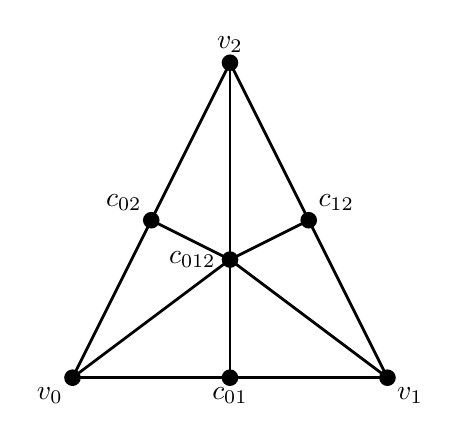
\begin{tikzpicture}[>=latex, scale=2]
          % Coords
          \coordinate (V0) at (0,0);
          \coordinate (V1) at (2,0);
          \coordinate (V2) at (1,2);
          \coordinate (C01) at (1,0);
          \coordinate (C02) at (0.5,1);
          \coordinate (C12) at (1.5,1);
          \coordinate (C) at (1,0.75);
          % Arrows
          \draw[line width=1pt]
            (V0) -- (V1);
          \draw[line width=1pt]
            (V1) -- (V2);
          \draw[line width=1pt]
            (V2) -- (V0);
          \draw[line width=1pt]
            (V0) -- (C);
          \draw[line width=1pt]
            (V1) -- (C);
          \draw[line width=1pt]
            (V2) -- (C);
          \draw[line width=1pt]
            (C01) -- (C);
          \draw[line width=1pt]
            (C02) -- (C);
          \draw[line width=1pt]
            (C12) -- (C);
          % Points
          \fill (V0) node[below left] {\( v_{0} \)} circle (1.5pt);
          \fill (V1) node[below right] {\( v_{1} \)} circle (1.5pt);
          \fill (V2) node[above] {\( v_{2} \)} circle (1.5pt);
          \fill (C01) node[below] {\( c_{01} \)} circle (1.5pt);
          \fill (C02) node[above left] {\( c_{02} \)} circle (1.5pt);
          \fill (C12) node[above right] {\( c_{12} \)} circle (1.5pt);
          \fill (C) node[left] {\( c_{012}\,\)} circle (1.5pt);
        \end{tikzpicture}
        \caption[Bsp. Umkreismittelpunktunterteilung]{Umkreismittelpunktunterteilung eines Dreieckelements \( v_{0}v_{1}v_{2} \) mit dessen Kanten und Ecken,
                                                      wobei \( c_{v_{1}\ldots v_{p}}:=c\left( v_{1}\ldots v_{p} \right) \)}
        \label{figCSDDreieck}
      \end{minipage}
      \hfill
      \begin{minipage}[t]{0.45\textwidth}
        \centering
        \begin{tikzpicture}[scale=2, >=latex]
          % Coords
          \coordinate (V0) at (0,0);
          \coordinate (V1) at (2,0);
          \coordinate (V2) at (1,2);
          \coordinate (C01) at (1,0);
          \coordinate (C) at (1,0.75);
          \coordinate (VV0) at (0,-0.3);
          \coordinate (VV1) at (2,-0.3);
          % Arrows
          \draw[line width=1pt, ->]
            (V0) -- node[below]{\( +1 \)} (C01);
          \draw[line width=1pt, ->]
            (V1) -- node[below]{\( -1 \)} (C01);
          \draw[line width=1pt, ->]
            (V1) -- (V2);
          \draw[line width=1pt, ->]
            (V2) -- (V0);
          \draw[line width=1pt, ->]
            (V0) -- (C);
          \draw[line width=1pt, ->]
            (V1) -- (C);
          \draw[line width=1pt, ->]
            (C01) -- (C);
          \draw[line width=1pt, ->]
            (VV0) -- (VV1);
          \draw[line width=1pt, style=dotted]
            (V0) -- (VV0);
          \draw[line width=1pt, style=dotted]
            (V1) -- (VV1);
          % Points
          \fill (V0) node[left] {\( v_{0} \)} circle (1.5pt);
          \fill (V1) node[right] {\( v_{1} \)} circle (1.5pt);
          \fill (V2) node[above] {\( v_{2} \)} circle (1.5pt);
          \fill (C01) node[below] {\( c_{01} \)} circle (1.5pt);
          \fill (C) node[above] {\( c_{012}\)} circle (1.5pt);
          \fill (VV0) node[left] {\( v_{0} \)} circle (1.5pt);
          \fill (VV1) node[right] {\( v_{1} \)} circle (1.5pt);
          % circ arrow
          \coordinate (CC) at (1,1.25);
          \def\r{0.2} 
          \draw[line width=1pt, ->] ($(CC)+(135:\r)$) arc (135:405:\r) -- ++ (-3pt,3pt);
          % circ arrow
          \coordinate (CC) at (0.75,0.25);
          \fill (CC) node[] {\small\(+1\)};
          \def\r{0.15} 
          \draw[line width=1pt, ->] ($(CC)+(135:\r)$) arc (135:405:\r) -- ++ (-3pt,3pt);
          % circ arrow
          \coordinate (CC) at (1.25,0.25);
          \fill (CC) node[] {\small\(-1\)};
          \def\r{0.15} 
          \draw[line width=1pt, ->] ($(CC)+(405:\r)$) arc (405:135:\r) -- ++ (3pt,3pt);
        \end{tikzpicture}
        \caption[Bsp. induzierte Orientierung]{ Wie wir sehen, ist
                                               \( \sgn_{\left[ v_{0},v_{1} \right]}\left( [ c_{01},c_{012} ] \right) = +1 \),
                                               dabei spielt es keine Rolle, ob wir \( v_{0} \prec \left[ v_{0},v_{1} \right] \)
                                               oder \( v_{1} \prec \left[ v_{0}, v_{1} \right] \) für die Berechnung hinzuziehen.}
        \label{figIndOrientDualKante}
      \end{minipage}
    \end{figure}
    Definition \ref{defIndOriElemDual} ist wohldefiniert, das heißt unabhängig von den gewählten \( \sigma^{i} \prec \sigma^{p} \).
    Denn würden wir ein \( \sigma^{i} \) durch ein \( \tilde{\sigma}^{i} \prec \sigma^{p} \) austauschen und es ändert sich dabei die Orientierung für das resultierende
    \(\left[ c(\sigma^{0}),\ldots,c(\tilde{\sigma}^{i}), \ldots, c(\sigma^{p}) \right] \), dann würde sich auch bei 
    \(\left[ c(\sigma^{0}),\ldots,c(\tilde{\sigma}^{i}), \ldots, c(\sigma^{n}) \right] \) die Orientierung ändern. 
    Das gilt natürlich für jedes beliebige \( \tilde{\sigma}^{i} \prec \sigma^{p} \) und auch für beliebig häufiges wiederholen der Wechsel.
    
    In Abbildung \ref{figIndOrientDualKante} ist beispielhaft die Berechnung der induzierten Orientierung für eine elementare 
    Dualkante in einem Dreieckelement dargestellt. 

  \begin{fazit}
    Damit wäre nun das geometrische Fundament für ein DEC gelegt, welches für diese Arbeit hier vollkommen ausreichend ist.
    Wenn wir genau hinschauen, ist zu bemerken, dass nicht alle Simplizes des Dualgitters vom Primärgitter nach unseren Definitionen eine induzierte Orientierung erhalten können.
    Wohl aber für eine Teilmenge des \( \csd K \), mehr als diese Teilmenge wird auch für die
    numerischen Schematas nicht vonnöten sein, wie wir noch sehen werden.
    
    Leider ist gerade die Wohlzentriertheit eine problematische Bedingung für die Zulässig\-keit von Gittern.
    Zum Beispiel gibt es in der FEM diese Anforderung nicht, obgleich wohlzentrierte Gitter die numerischen Eigenschaften sicherlich verbessern würden.
    In \ref{secGittergenerierung} wird ein einfacher Ansatz geboten für den DEC brauchbare Triangulierungen aus nicht zulässigen Gittern zu generieren.
    Jedoch setzt das auch einiges explizites oder implizites Wissen an die tatsächliche Geometrie der Mannigfaltigkeit voraus und es muss zusätzliche Rechnergestützte Arbeit in das Problem
    gesteckt werden. Damit zeichnet sich schon hier das größte Manko eines DECs auf wohlzentrierten Primärgittern ab.
    In zukünftigen Arbeiten muss die Wohlzentriertheit abgeschwächt werden.
    Ein kleiner Sieg wäre zum Beispiel schon eine "`Wohlzentriertheit im Limes"', das heißt es wären auch Umkreismittelpunkte auf dem Rand eines Simplexes zulässig.
    Damit wären auf zweidimensionalen Gittern auch Rechtecke möglich und folglich auch, selbst im planaren, Ecken mit nur 4 Dreieckelementen, die sich diese Ecke teilen.
    Prinzipiell könnte so auch der hier vorgestellte DEC in gleicher Art und Weise geführt werden. 
    Allerdings können sich so auch Kanten der Länge null ergeben und somit müssten wir auch
    ständig aufpassen in den späteren Berechnungs\-schematas nicht durch null zuteilen. 
    Aus diesem Grund sehen wir hier in dieser Arbeit davon ab.
    In \ref{secImpliziteMannigfaltigkeiten} wird auch noch kurz gezeigt wie wir numerisch mit implizit gegebenen Oberflächen umgehen können.

    Eine weitere Möglichkeit ist es einen ganz anderen Ansatz für die Dualität der Gitter zu verfolgen.
    In \cite{sensen} wird im Rahmen einer diskreten Chern-Simons-Theorie auf speziellen dreidimensionalen Mannigfaltigkeiten (Raumzeit) eine baryzentrische Unterteilung genutzt.
    Das heißt der Mittelpunkt ist hier das "`Massezentrum"'.
    So gilt zum Beispiel \( c\left( \left[ v_{0},v_{1},v_{2} \right] \right) = \frac{1}{3}\sum_{i=0}^{2}v_{i}\).
    Die Diskretisierung des Hodge-Stern-Operators in einem allgemeinen DEC-Kontext würde somit aber ziemlich schwierig werden, da hier auch metrische Informationen mit eingehen.
    Die Tatsache, dass bei einer Umkreismittelpunktunterteilung die zueinander dualen Simplizes im gewissen Sinne orthogonal sind, 
    macht es uns da später einfacher.
    Für zukünftige Arbeiten sollte dennoch die baryzentrische Dualität ein paar Gedanken wert sein, denn jeder Simplizialkomplex ist mit dieser Unterteilung baryzentrisch wohlzentriert,
    speziell auch das Dualgitter selbst. 
    Das gibt die Umkreismittelpunktunterteilung nicht her. 
    Somit würde auch einer globalen und sogar lokalen Verfeinerung bzgl. der Zulässigkeit des Gitters nichts mehr im Wege stehen.
  \end{fazit}









\section{Kettenkomplexe}

  \begin{ziel}
    Ziel dieses Abschnittes ist es, die zuvor eingeführten Simplizes in einer algebraisch sinnvollen Weise zu "`verketten"'.
    Die Universaleigenschaft sichert uns zudem, dass wir Operatoren auf diesen "`Ketten"' nur auf den einzelnen Simplizes definieren
    müssen, da sie sich kanonisch auf den "`Ketten"' fortsetzen lassen.
    Im Mittelpunkt sollen hier der Sternoperator, der Simplizes mit ihren dualen "`Ketten"' identifiziert et vice versa,
    und der Randoperator, der den Ketten und speziell auch den Simplizes die Komplexeigenschaft bringt, stehen.
  \end{ziel}

  \begin{definition}
    Eine \( p \)-Kette ist eine formale Summe aus \( p \)-Simplizes mit Koeffizienten in \( \Z \),
    das heißt für einen Simplizialkomplex \( K \) ist
    \begin{align}
      \label{eqKette}
      C_{p}(K) &:= \left\{\sum_{\sigma\in K^{(p)}}a_{\sigma}\sigma \middle| a_{\sigma}\in\Z \right\}
    \end{align}
    die Menge aller \( p \)-Ketten über \( K \).
  \end{definition}
  Prinzipiell würden für das reine Rechnen mit \( p \)-Ketten Koeffizienten aus \( \left\{ +1, 0,  -1 \right\} \) ausreichen,
  da wir Simplizes gleicher Dimension immer nur "`aneinander reihen"' (konkatenieren) werden. 
  Das entspräche dem reinen Addieren (\( +1 \)) zweier benachbarter Simplizes.
  Subtrahieren (\( -1 \)) erlaubt zudem die Orientierung, falls vorhanden, zu wechseln.
  Auch Koeffizienten aus \( \R \) sind denkbar, dann wäre \( C_{p}(K) \) ein \( \R \)-Vektorraum.
  Dass wir hier jedoch \( \Z \) gewählt haben, hat den Vorteil, dass \( C_{p}(K) \) abzählbar und bezüglich der Addition eine freie abelsche Gruppe ist
  (mit Erzeugendensystem \( K^{(p)} \), d.h.  \( \left\langle K^{(p)} \right\rangle_{C_{p}(K)} = C_{p}(K) \)),
  in der die Universaleigenschaft gilt.
  Genauer, \( C_{p}(K) \) ist frei bzgl. jeder abelschen Gruppe \( \mathfrak{A} \), deswegen kommutiert das Diagramm
  \begin{align}
    \label{diagFreieAbelscheGruppe}
    \begin{xy}
      \xymatrix{
        C_{p}(K) \ar[rd]^{\widehat{op}} & \\
        K^{(p)} \ar@^{(->}[u] \ar[r]_{op}& \mathfrak{A}
      }
    \end{xy}
  \end{align}
  mit \( op = \widehat{op}|_{K^{(p)}} \), das heißt \( \widehat{op} \) ist der eindeutig bestimmte Homomorphismus, der \( op \) fortsetzt.
  Und zwar gilt
  \begin{align}
    \widehat{op}\left(\sum_{\sigma\in K^{(p)}}a_{\sigma}\sigma\right) = \sum_{\sigma\in K^{(p)}}a_{\sigma}op(\sigma) \formpunkt
  \end{align}
  Somit reicht es vollkommen aus, dass wir bestimmte Operatoren/Homomorphismen nur auf der Basis definieren und diese dann linear fortsetzen.
  Speziell werden wir uns das noch für \( \mathfrak{A} = C_{q}(\csd K) \), \( C_{q}(K) \), \( \R \) oder \( \hom(C_{p}(K),\R) \) zunutze machen. 

  Geometrisch kann die in \eqref{eqKette} rein formale Addition als Vereinigung interpretiert werden. 
  In Definition \ref{defDualZelle} wurde die Dualzelle eines \( p \)-Simplex eingeführt. 
  Sie ist die geometrische Vereinigung von \( (n-p) \)-Simplizes.
  Nun liegt es nahe, diese Dualzelle als \( (n-p) \)-Kette darzustellen.
  Das führt uns zur Definition des Sternoperators.

  \begin{definition}
     Es sei \( K \) ein wohlzentriertes Primärgitter der Dimension \( n \).
     Der Sternoperator \( \star: C_{p}(K) \rightarrow   C_{n-p}(\csd K) \) ist definiert durch
     \begin{align}
       \star\sigma^{p} := \sum_{\sigma^{p} \prec \sigma^{p+1} \prec \ldots \prec \sigma^{n}}
                                                   s_{\sigma^{p}, \sigma^{p+1}, \ldots, \sigma^{n}} \left[ c(\sigma^{p}), c(\sigma^{p+1}), \ldots, c(\sigma^{n}) \right]
     \end{align}
     mit \( s_{\sigma^{p}, \sigma^{p+1}, \ldots, \sigma^{n}} \in \left\{ -1,+1 \right\}\) so gewählt, dass  
     \( s_{\sigma^{p}, \sigma^{p+1}, \ldots, \sigma^{n}} \left[ c(\sigma^{p}), c(\sigma^{p+1}), \ldots, c(\sigma^{n}) \right] \) der
     durch \( \sigma^{p} \) induzierte Orientierung entspricht.
  \end{definition}
  Wie man sieht, besteht das Bild von \( \star \) nur aus Verkettungen von elementaren Dualsimplizes und freilich ist das eine Untergruppe des \( C_{n-p}(\csd K) \).
  Wir definieren deshalb hier \( C_{n-p}(\star K) := Im(\star_{(p)}) = \star C_{p}(K) \).
  Also gilt \( \star: C_{p}(K) \rightarrow   C_{n-p}(\star K) \).

  Wir können somit Simplizes verketten und haben mit dem Sternoperator auch einen Isomorphismus
  zwischen den Ketten des Primär- und elementaren Dualgitters.
  Die Surjektivität ist per Definition gegeben, da \( C_{n-p}(\star K) \) Bild ist.
  Für
  \begin{align}
    0 &= \star \sum_{\sigma \in K^{(p)}} a_{\sigma}\sigma = \sum_{\sigma \in K^{(p)}} a_{\sigma} \left( \star\sigma\right)
  \end{align}
  ergibt sich über Koeffizientenvergleich nur der triviale Kern \( \left\{ 0 \right\} \) für den Gruppenhomomorphismus \( \star \), 
  folglich ist der Sternoperator auch injektiv.
  
  Des Weiteren ist auch \( C_{n-p}(\star K) \) freie abelsche Gruppe mit 
  \mbox{\( \star K^{(n-p)} := \star\left( K^{(p)} \right) \)} als Erzeugendensystem, 
  denn für jedes \( \hat{c} = \star c \in C_{n-p}(\star K) \) mit \( c = \sum_{\sigma \in K^{(p)}} a_{\sigma}\sigma \in C_{p}(K) \) für gewisse \( a_{\sigma} \in \Z \) gilt
  \begin{align}
    \label{eqSternSigmaKette}
    \hat{c} &= \star \sum_{\sigma \in K^{(p)}} a_{\sigma}\sigma
             = \sum_{\sigma \in K^{(p)}} a_{\sigma} \left( \star\sigma\right)
             = \sum_{\hat{\sigma}:=\left( \star\sigma\right) \in \star K^{(p)} } a_{\sigma} \hat{\sigma} \formpunkt
  \end{align}
  Somit ist \(\star K^{(n-p)}  \) Erzeugendensystem und falls \( \hat{c} = \star c = 0 \), 
  dann muss auch \( c = 0 \) gelten, weil der Sternoperator ein Gruppenisomorphismus ist,
  das heißt es wären alle \( a_{\sigma} = 0 \) in \eqref{eqSternSigmaKette} als einzige (triviale) Lösung für \( \hat{c} = 0 \).
  Genauso wie bei \eqref{diagFreieAbelscheGruppe} können wir nun Operatoren auf \( C_{n-p}(\star K) \) auf der Basis \( \star K^{(n-p)} \) definieren und fortsetzen, 
  wenn der Operator auf eine abelsche Gruppe abgebildet wird.

  Da der Sternoperator das simpliziale Analogon zum Hodge-Stern-Operator \( * \) werden soll, sollten auch analoge, also auf syntaktischer Ebene gleiche, Bedingungen gelten.
  Für eine Differentialform \( \alpha\in\Omega^{p}(M) \) auf einer \( n \)-dimensionalen Mannigfaltigkeit \( M \) gilt 
  (vgl. \cite[ Kap.6.2.]{Marsden}\footnote{Der Index, der von uns behandelten Mannigfaltigkeiten, ist immer null.})
  \begin{align}
    **\alpha &= (-1)^{p(n-p)}\alpha \formpunkt
  \end{align}
  Deswegen definieren wir den Sternoperator auf \( C_{p}(\star K) \) implizit über genau diese Bedingung.

  \begin{definition}
    \label{defDoppelSternBedingung}
    Es sei \( K \) ein wohlzentriertes Primärgitter der Dimension \( n \).
    Der (duale) Sternoperator \( \star: C_{p}(\star K) \rightarrow   C_{n-p}(K) \) definiert sich über
    \begin{align}
      \label{eqDoppelSternBedingung}
      \star\star \sigma^{n-p} &= (-1)^{p(n-p)}\sigma^{n-p}
    \end{align}
    für alle \( \sigma^{n-p} \in C_{n-p}(K) \).
  \end{definition}
  Natürlich gilt Bedingung \eqref{eqDoppelSternBedingung} auch für alle Ketten \( \star\sigma^{n-p} =: \hat{\sigma}^{p} \in C_{p}(\star K)\), denn
  \begin{align}
    \begin{aligned}
    \star\star\hat{\sigma}^{p} &= \star\star\star\sigma^{n-p} = \star\left((-1)^{p(n-p)}\sigma^{n-p}\right)
                                = (-1)^{p(n-p)}\star\sigma^{n-p} \\
                                &=  (-1)^{p(n-p)}\hat{\sigma}^{p} \formpunkt
    \end{aligned}
  \end{align}

  \begin{bemerkung}
    Es sei \( K \) ein zweidimensionales wohlzentriertes Primärgitter ohne Rand,
    dann wird mit dem Sternoperator
    \begin{itemize}
      \item ein Knoten auf eine 2-Kette abgebildet, sodass alle Dreiecke in dieser Verkettung vorkommen, die diesen Knoten als Ecke haben, 
            et vice versa.
            Die Orientierung der Flächenelemente ist die aller Flächenelemente. 
            Die sich ergebene 2-Kette nennen wir auch Voronoi-Zelle.
      \item eine Kante \( \sigma^{1} \) auf eine 1-Kette abgebildet, die aus genau den beiden dualen Kanten des \( \csd K \) besteht, die \( c(\sigma^{1}) \) als gemeinsamen Randpunkt
            haben, et vice versa.
            Die sich ergebene 1-Kette nennen wir auch Voronoi-Kante. 
            Die orientierte Kante bzw. Voronoi-Kante wird somit immer in Richtung der Flächenorientierungen "`gedreht"'.
      \item ein Dreieckelement auf dessen Umkreismittelpunkt abgebildet, et vice versa. 
            Deswegen nennen wir den Umkreismittelpunkt auch Voronoi-Knoten.
    \end{itemize}
    In Abbildung \ref{figBspSternoperator2D} ist dieser Zusammenhang für einen Ausschnitt eines Primärgitters beispielhaft dargestellt.
  \end{bemerkung}

  \begin{figure}
    \centering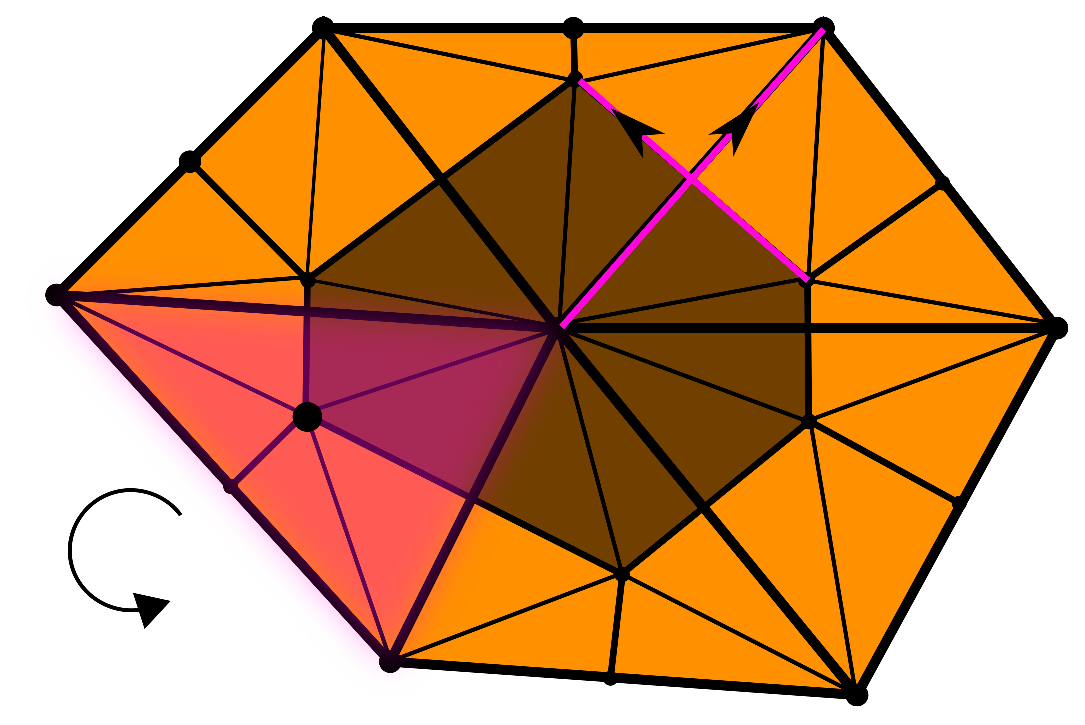
\includegraphics[width=0.8\textwidth]{bilder/dualSigma0.eps}
    \caption[Bsp. Sternoperator in 2D]{Beispiel für den Sternoperator auf einem Primärgitter der Dimension 2.
                                       Für Knoten und Volumenelemente ändert sich die Orientierung auch nach mehrmaliger Anwendung nicht.
                                       Dagegen muss bei Kanten immer gegen den Uhrzeigersinn "`gedreht"' werden, sodass z.B. \( \star\star\sigma^{1} = -\sigma^{1} \) gilt.}
    \label{figBspSternoperator2D}
    \vspace{1cm}
    \centering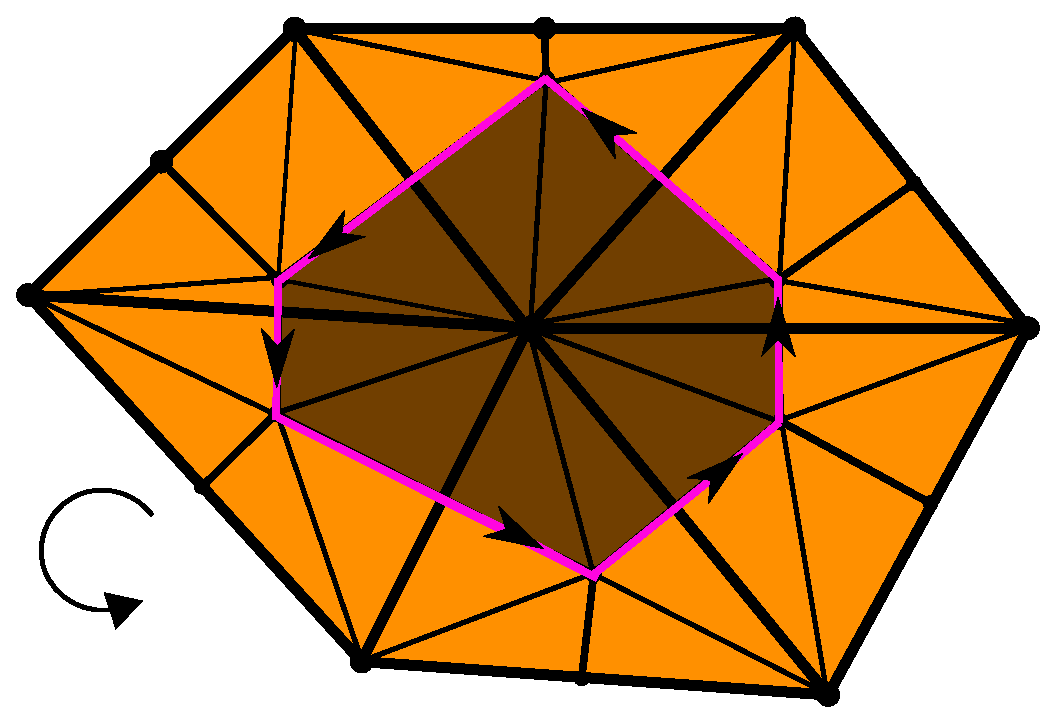
\includegraphics[width=0.8\textwidth]{bilder/dualSigmaRand.eps}
    \caption[Bsp. Randoperator auf (dualen) 2-Kette]{Rand mit Orientierungen einer (dualen) 2-Kette, genauer, der Voronoi-Zelle, der primären Ecke in der Mitte des Simplizialkomplexes.
                                                     Es ergibt sich eine (duale) 1-Kette aus Voronoi-Kanten, dual zu den primären Kanten, die sich im Mittelpunkt treffen.
                                                     Die Orientierung dieser primären Kanten muss für die Berechnung so geändert werden, dass sie alle nach außen zeigen.}
    \label{figBspRandAufDualZelle}
  \end{figure}

  Nun wird es Zeit der Überschrift Rechnung zu tragen und einen Operator einzuführen, der die Komplexeigenschaft erfüllt. 
  
  \begin{definition}
    \label{defRandoperator}
    Es sei \( K \) ein Simplizialkomplex und \( 0 < p \le n \).
    Der Randoperator \( \partial_{p}: C_{p}(K) \rightarrow C_{p-1}(K) \) definiert sich durch
    \begin{align}
      \partial_{p}\sigma^{p} := \sum_{i=0}^{p} (-1)^{i} \left[ v_{0}, v_{1}, \ldots, \hat{v}_{i}, \ldots, v_{p} \right]
    \end{align}
    wobei \( \sigma^{p} = \left[ v_{0}, v_{1}, \ldots, v_{p} \right] \in K\) ist. 
    Das Dach bedeutet wieder, dass die entsprechende Ecke weggelassen wird.
    Da schon vorher erwähnt wurde, dass Knoten offene Mengen bezüglich der simplizialen Topologie sind, setzen wir konsistenterweise
    \begin{align}
      \partial_{0}\sigma^{0} := 0
    \end{align}
    Wenn kein Grund zur Verwirrung besteht, dann darf auch nur \( \partial \) statt \( \partial_{p} \) geschrieben werden.
  \end{definition}

  \begin{folgerung}
    Der (duale) Randoperator \( \partial_{p}: C_{p}(\star K) \rightarrow C_{p-1}(\star K) \) lässt sich vom obigen Randoperator für einen wohlzentrierten Simplizialkomplex \( K \) ableiten, 
    indem wir \( \csd K \) als Simplizialkomplex nutzen und den Operator auf \( C_{p}(\star K) \le C_{p}(\csd K) \) einschränken.
    Das bedeutet für \( \hat{\sigma}^{p} = \star\sigma^{n-p} \in \star K^{(p)} \) (\( \star K^{(p)} \) Erzeugendensystem)
    \begin{align}
      \partial_{p} \hat{\sigma}^{p} &= \partial_{p}\star\sigma^{n-p} \\
                                    &= \sum_{\sigma^{n-p+1} \succ \sigma^{n-p}} \star \left( s_{\sigma^{n-p+1}} \sigma^{n-p+1} \right) \formkomma
    \end{align}
    wobei \( s_{\sigma^{n-p+1}} \in \left\{ -1,+1 \right\} \) so gewählt wird, dass die durch \( s_{\sigma^{n-p+1}} \sigma^{n-p+1} \) induzierte Orientierung für
    \( \sigma^{n-p} \) konsistent ist. (vergleiche Beispiel in Abbildung \ref{figBspRandAufDualZelle})
  \end{folgerung}
  \begin{proof}
    Dass \( \partial_{p} C_{p}(\star K) \le C_{p-1}(\csd K) \) gilt, ist klar, wegen der Untergruppeneigenschaft von \( C_{p}(\star K) \) und weil der Randoperator ein Homomorphismus ist.
    Zu zeigen ist allerdings noch, dass \( \partial_{p} C_{p}(\star K) \le C_{p-1}(\star K) \) gilt. 
    Dabei reicht es auch hier aus, dies nur auf dem Erzeugendensystem zu zeigen (algebraischer Induktionsanfang).
    Der (algebraische) Induktionsschritt gilt dann immer wegen der Universaleigenschaft für homomorphe Fortsetzungen auf freie abelsche Gruppen.

    Für eine bessere Lesbarkeit substituieren wir den Grad der Simplizes \( (n-p) \leftrightarrow p \) und schreiben nur \( s \) für \( s_{\bullet} \in \left\{ +1,-1 \right\} \)
    und machen uns dabei bewusst, dass der Koeffizient \( s \) in jeder Zeile und Summanden etwas anderes bedeuten kann.
    {\allowdisplaybreaks
    \begin{align}
      \partial_{n-p}\star\sigma^{p} &= \sum_{\sigma^{p}\prec\ldots\prec\sigma^{n}} s \partial_{n-p} \left[ c(\sigma^{p}), c(\sigma^{p+1}),\ldots, c(\sigma^{n})\right] \label{eqproof1}\\
                              &= \sum_{\sigma^{p}\prec\ldots\prec\sigma^{n}} s 
                                          \sum_{i=p}^{n} (-1)^{i-p} \left[ c(\sigma^{p}),\ldots, \widehat{c(\sigma^{i})},\ldots, c(\sigma^{n})\right] \label{eqproof2}\\
                              &= \sum_{\sigma^{p}\prec\ldots\prec\widehat{\sigma^{k}}\prec\ldots\prec\sigma^{n}} s
                                          \sum_{i=p}^{n} (-1)^{i-p} 
                              \left(\begin{aligned}
                                            \phantom{-}\left[ c(\sigma^{p}),\ldots, c(\sigma_{1}^{k}),\ldots,\widehat{c(\sigma^{i})},\ldots, c(\sigma^{n})\right] \\
                                                     - \left[ c(\sigma^{p}),\ldots, c(\sigma_{2}^{k}),\ldots,\widehat{c(\sigma^{i})},\ldots, c(\sigma^{n})\right]
                              \end{aligned}\right) \label{eqproof3}\\
                              &= \sum_{\sigma^{p}\prec\ldots\prec\sigma^{n}} s 
                                          \sum_{\begin{smallmatrix}
                                                  i & = & p \\
                                                  i & \neq & k
                                                \end{smallmatrix}}^{n} (-1)^{i-p} \left[ c(\sigma^{p}),\ldots, \widehat{c(\sigma^{i})},\ldots, c(\sigma^{n})\right] \label{eqproof4}\\
                              &\hphantom{=}\vdots\notag\\
                              &= \sum_{\sigma^{p}\prec\ldots\prec\sigma^{n}} s \left[ c(\sigma^{p+1}), c(\sigma^{p+1}),\ldots, c(\sigma^{n})\right]  \label{eqproof5}\\
                              &= \sum_{\sigma^{p}\prec\sigma^{p+1}}
                                          \sum_{\sigma^{p+1}\prec\ldots\prec\sigma^{n}} s \left[ c(\sigma^{p+1}), c(\sigma^{p+1}),\ldots, c(\sigma^{n})\right]  \label{eqproof5}\\
                              &= \sum_{\sigma^{p+1} \succ \sigma^{p}} \star \left( s \sigma^{p+1} \right) \in C_{n-p-1}(\star K)
    \end{align}}
    Dabei ergibt sich \eqref{eqproof1} aus der Homomorphie des Randoperators und \eqref{eqproof2} nach Definition \ref{defRandoperator}.
    In \eqref{eqproof3} schreiben wir die beiden Summanden für \( \sigma^{k}_{r} \) für \( r = 1,2 \) explizit aus. 
    Es gibt immer genau zwei solcher Folgen 
    \begin{align}
      \sigma^{p}\prec\ldots\prec\sigma^{k-1}\prec\sigma^{k}\prec\sigma^{k+1}\prec\ldots\prec\sigma^{n}\formkomma
    \end{align}
    wenn bis auf \( \sigma^{k} \) und \( \sigma^{p} \) alle Simplizes fest gewählt sind. 
    Die beiden sich ergebenden, dualen Simplizes sind gegensätzlich orientiert, da die "`Zählrichtung"' der Dualecken anders herum ist.
    \eqref{eqproof4} folgt daraus, dass sich beide Summanden für \( i=k \) aufheben. 
    Das machen wir dann für alle \( p < k \le n \).
    Der Rest ergibt sich durch aufteilen der Summe und der Definition des Sternoperators.

    Bemerkung:
    In z.B. \cite{hirani} wurde der duale Randoperator per Definition festgelegt ohne zu prüfen oder zu verweisen 
    ob er mit dem primären Randoperator auf dualen Gittern konsistent ist.
    Dem wurde hier nun Genüge getan. Es ist der gleiche Operator mit eingeschränktem Definitionsbereich.
  \end{proof}

  \begin{folgerung}
    \label{folgSimplizialerKettenkomplex}
    Die Folgen \( \left( C_{p}(K), \partial_{p} \right)_{0 \le p \le n} \) beziehungsweise \( \left( C_{p}(*K), \partial_{p} \right)_{0 \le p \le n} \) 
    bilden einen (simplizialen) Kettenkomplex.
    \begin{align}
      \begin{xy}
        \xymatrix{
          0 \ar[r] & 
          C_{n}(K) \ar[r]^{\partial_{n}} \ar[d]^{\star} & 
          C_{n-1}(K) \ar[r]^{\partial_{n-1}} \ar[d]^{\star} & 
          \ldots \ar[r]^{\partial_{1}} & 
          C_{0}(K) \ar[r] \ar[d]^{\star} &
          0 \\
          0  & 
          C_{0}(\star K) \ar[l] & 
          C_{1}( \star K) \ar[l]^{\partial_{1}} & 
          \ldots \ar[l]^{\partial_{2}} & 
          C_{n}(\star K) \ar[l]^{\partial_{n}} &
          0 \ar[l]
        }
      \end{xy}
    \end{align}
    Das heißt \( \partial_{p} \circ \partial_{p+1} = 0\), was sich einfach nachrechnen lässt.
    Zudem sei noch der Isomorphismus \( \star \) im Diagramm mit angegeben.
  \end{folgerung}

    
  \begin{fazit}
    Am Anfang des Absatzes haben wir uns entschieden, die Koeffizienten der Ketten aus \( \Z \) zu wählen.
    Hätten wir \( \R \) genommen, dann wäre \( C_{p}(K) \) ein \( \R \)-Vektorraum mit (linear unabhängiger) Basis \( K^{(p)} \).
    Dementsprechend würde auch immer noch alles aus diesem Absatz gelten.
    Wir würden aber die Abzählbarkeit des \( C_{p}(K) \) aufgeben, die uns unter Umständen später noch von Nutzen sein könnte.

    Wenn wir allgemein \( C_{p} \) als Funktor auf der Kategorie der Simplizialkomplexe sehen, also
    \begin{align}
      \begin{xy}
        \xymatrix{
          C_{p}(K) \ar[r]^{C_{p}(f)} & C_{p}(\mathfrak{S}) \\
          K \ar@{|->}[u]^{C_{p}} \ar[r]_{f} & \mathfrak{S} \ar@{|->}[u]_{C_{p}}
        }
      \end{xy}
    \end{align}
    dann wäre
    \begin{align}
      f_{p} &:= C_{p}(f): \sum_{\sigma\in K^{(p)}} a_{i}\sigma \mapsto \sum_{\sigma\in K^{(p)}} a_{i}f(\sigma)
    \end{align}
    kanonisch gegeben. 
    Somit wäre zum einen eine Zuordnung zu den singulären Kettenkomplexen mit 
    \begin{align}
      f := \left\langle \bullet, \bullet \right\rangle := K \rightarrow K_{sing} 
                                                           : \left[ v_{0},\ldots v_{p}\right] \mapsto \left\langle \bullet , \left[ v_{0},\ldots v_{p}\right] \right\rangle
                                                           := \left( \left[ \mu^{0},\ldots,\mu^{p} \right] \mapsto \sum_{i=0}^{p} \mu^{i} v_{i}\right)
    \end{align}
    oder zu den abstrakten Kettenkomplexen mit \( f:=\pi \) (Projektion/Ankleben der Simplizes auf die Mannigfaltigkeit) gegeben.
    Zum anderen haben wir in zukünftigen Arbeiten auch die Möglichkeit Oberflächen zu betrachten, die sich zeitlich ändern 
    (\( f(t):K\rightarrow K(t) \)) unter beibehalten der simplizialen Struktur, so es denn möglich ist.
    Im Einzelnen muss dann noch geprüft werden, unter welchen Voraussetzungen \( f\circ\partial = \partial\circ f\) beziehungsweise \( f\circ\star = \star\circ f\) gilt.
  \end{fazit}
  




\section{Gittergenerierung für Oberflächen}
\label{secGittergenerierung}


  \begin{ziel}
    Die Wohlzentriertheit eines Gitters ist Pflicht, da ohne sie kein brauchbares duales Gitter (Voronoi-Gitter) erzeugt werden kann. 
    Diese zur Triangulierung duale Gebietsdiskretisierung wird aber benötigt, um zum Beispiel einen 
    diskreten Hodge-Stern-Operator sinnvoll zu entwickeln. 
    Bei einem nicht wohlzentrierten Dreieck liegt der Voronoi-Knoten \( \star\sigma^{2} \) nicht im Dreieck \( \sigma^{2} \).
    Das Problem dabei ist, dass sich die Werte auf \( \star\sigma^{2} \) und \( \sigma^{2} \) nur um einen 
    metrischen Faktor\footnote{hier \( |\sigma^{2}| \) bzw. dessen Reziproke} unterscheiden sollten.
    Diese Voraussetzung wäre aber nicht mehr haltbar, da die Gebiete, die beide Elemente einnehmen, disjunkt sind. 
    Sie können sogar  "`sehr weit"'
    von einander entfernt liegen.
    Dann hätte die eine Größe fast nichts mehr mit der anderen gemein und die Linearität beider wäre nicht mehr gegeben.

    Wohlzentriertheit ist eine schwerwiegende Einschränkung an die Gitterstruktur. Sie verbietet unter anderem einen 1-Ring um einen Knoten
    aus vier oder weniger Dreieckelementen.
    Für eine nicht planare Triangulierung mit positiver Gaußkrümmung mag ein 1-Ring aus vier Flächenelementen gerade noch funktionieren, da die Innenwinkelsumme der inneren Kanten weniger als \( 2\pi \) ist.
    Im planaren Fall erhalten wir aber für eine optimale\footnote{bzgl. der maximalen Winkel} Triangulierung Winkel von \( \frac{\pi}{2} \) 
    und somit nur Wohlzentriertheit im Limes\footnote{für planare äquidistante Gitter kann diese schwächere Restriktion dennoch sinnvoll sein, da somit bekannte Differenzenschematas entstehen können}.
    Damit sind oft genutzte lokale und globale Strategien zur Verfeinerung nicht anwendbar. 
    So wird zum Beispiel bei der FEM-Toolbox AMDiS \cite{amdis} die längste Kante halbiert und von dort zwei neue Kanten zu den jeweils gegenüberliegenden Knoten der beiden angrenzenden Dreiecken erstellt. Der neu entstandene Knotenpunkt hat folglich einen 1-Ring aus 4 Flächenelementen.
    Auch CAD-Programme liefern im Allgemeinen keine geeigneten Gitter. 
    Ein möglicher Ausweg könnte eine Triangulierung (bzw. Neutriangulierung) mittels angepasstem Delaunay oder anderen Algorithmen sein, zum Beispiel Centroidal Voronoi Tessellation (CVT)\cite{CVTGunzburger}, 
    Optimal Delaunay Triangulations (ODT)\cite{ODT} oder Hexagonal Delaunay Triangulation\cite{HDT}.

    Im Folgenden wollen wir davon ausgehen, dass zumindest eine Triangulation vorliegt, die die Bedingung erfüllt, dass jeder Knoten Teil von mehr als 4 Dreiecken ist. 
    Damit möchten wir ein Oberflächengitter erzeugen, welches wohlzentriert ist.
    Die Struktur des Simplizialkomplexes soll dabei erhalten bleiben. Nur die Knotenpunkte werden neu arrangiert. Das setzt natürlich voraus, dass die Oberfläche exakt, 
    zum Beispiel explizit durch eine Immersion \( X: M \rightarrow \R^{3} \) oder implizit durch das 0-Niveau einer Level-Set-Funktion\cite{levelset}, oder eine Approximation der 2-Mannigfaltigkeit höher als 1 gegeben ist.

    Ansätze zur Gitterverbesserung, bei der die Wohlzentriertheit im Vordergrund steht, gibt es bis jetzt wenige.
    Denn obwohl diese Forderung an der Triangulation für viele numerische Verfahren Vorteile bringen würde, 
    so ist sie doch nur für den hier verwendeten DEC zwingend. 
    Eine Arbeit ist zum Beispiel \cite{meshHirani}, wobei auch hier das diskrete Äußere Kalkül die Motivation bildete.
    Hier wird eine Kostenfunktion aufgestellt, deren Argument des Minimums ein wohlzentrierter Simplizialkomplex ist.
    Leider muss solch ein Minimum nicht existieren, weder im planaren noch auf gekrümmten Oberflächen.
    Wir wollen hier im Folgenden einen ähnlichen Ansatz verwenden. 
    Dazu sind Kraftvektoren an den Knoten gegeben, die das Gitter so unter Zwang setzen, dass die daraus resultierende Bewegung der
    Knoten, wenn es denn möglich ist, eine wohlzentrierte Triangulation formt. 
    Das Modell ist nicht neu und wird zum Beispiel zur Simulation von biologischem Zellgewebe verwendet. 
    Einen Überblick zu der Thematik bietet \cite{meshCooper}.  
  \end{ziel}

  
  
  \subsection{Mechanisches Modell und dessen Diskretisierung}
    
    Ein einfacher mechanischer Ansatz, um nach gewissen Kriterien ein optimales Gitter zu entwickeln, ist
    \begin{align}
      \gamma\frac{\d \vec{x}_{i}}{\d t} &= \vec{F}(\vec{x}_{i}) \formpunkt
      \label{visd}
    \end{align}
    Diese gewöhnliche Differentialgleichung erster Ordnung beschreibt eine Viskosedämpfung am Knoten 
    \( \sigma^{0}_{i} \) mit dem Koordinatenvektor \( \vec{x}_{i} \in M \subset \R^{3}\) und Viskositätskoeffizient \( \gamma \).
    Eine einfache Diskretisierung des Problems \eqref{visd} ist das explizite Eulerverfahren 
    mit nachgeschalteter Projektion \( \pi:\R^{3} \rightarrow M \) um die Nebenbedingung \( \vec{x}_{i} \in M \)
    zu erfüllen.
    \begin{align}
      \vec{x}_{i}(t+\Delta t) &= \pi\left(\vec{x}_{i}(t) + h \vec{F}_{i}\right) \formpunkt
      \label{euler}
    \end{align}
    Wobei \( h:= \frac{\Delta t}{\gamma} \) und \( \vec{F}_{i}:= \vec{F}(\vec{x}_{i}(t)) \).
    Der Kraftvektor \( \vec{F}_{i} \) resultiert aus Interaktionen mit den anderen Knoten. 
    Im Overlapping-Sphere-Modell(OS)\cite{meshCooper} sind das all die Knoten \( \sigma^{0}_{j} \), die einen bestimmten Abstand zu \( \sigma^{0}_{i} \) haben.
    Für das explizite Eulerverfahren (Verfahren 1.Ordnung) werden kleine Schrittweiten \( h \) benötigt. 
    Allerdings bringen Verfahren höherer Ordnung wahrscheinlich keine signifikant besseren Ergebnisse. Zum einen könnte eine größere Schrittweite
    nicht ausgenutzt werden, da es sonst passieren kann, dass sich, durch die resultierende größere Verschiebung eines Knoten, Dreiecke überlappen
    und somit keine zulässige Triangulierung mehr vorliegt. Zum anderen reduziert die Projektion \( \pi \) die Konvergenzordnung der Verfahren.
    So wurde zum Beispiel in den numerischen Experimenten auch das Heun-Verfahren (explizites Runge-Kutta-Verfahren der Ordnung 2) getestet, ohne
    nennenswerte bessere Resultate, dafür mit wesentlich höheren Kosten in der Berechnung.
    Implizite Verfahren haben einen zu hohen Aufwand in der Implementation, denn es ist zu bedenken, dass der Kraftvektor \(\vec{F}_{i}\) nicht
    nur von den Koordinaten \(  \vec{x}_{i} \) abhängt, sondern auch von der umgebenden Struktur.

    Wir wollen hier, im Gegensatz zum OS-Modell, die Gitterstruktur des Simplizialkomplexes ausnutzen, das heißt es interagieren genau die Knoten miteinander, die eine gemeinsame Kante besitzen. Somit lässt sich der Kraftvektor \( \vec{F}_{i} \) zerlegen zu
  \begin{align}
    \vec{F}_{i} &= \sum_{\sigma^{1}:=[\sigma^{0}_{j}, \sigma^{0}_{i}]\succ\sigma^{0}_{i}} 
                                  \frac{F_{\sigma^{0}_{i}\prec\sigma^{1}}}{\|\vec{x}_{j} - \vec{x}_{i}\|} \left(\vec{x}_{j} - \vec{x}_{i}\right)
    \formpunkt
  \end{align}
  \( F_{\sigma^{0}\prec\sigma^{1}} \) ist folglich die Kraft die am Knoten \( \sigma^{0} \) in Richtung der Kante \( \sigma^{1} \) wirkt. 
  Da die Kraft aber auch von der Geometrie der Flächenelemente abhängen kann, zerlegen wir die Kantenkräfte weiter zu
  \begin{align}
    F_{\sigma^{0}\prec\sigma^{1}} &= \sum_{\sigma^{2}\succ\sigma^{1}} F_{\sigma^{0}\prec\sigma^{1}\prec\sigma^{2}}
    \formpunkt
  \end{align}
  Als praktisch erweist es sich außerdem, die Kräfte dimensionslos zu halten, da somit eventuell auftretende Parameter für unterschiedliche
  Ausgangsgitter annähernd gleich gewählt werden können. 
  Die Schrittweite \( h \) in \eqref{euler} hängt somit annähernd linear von der Gitterweite ab. 
  Zu beachten ist hierbei, dass sich die Gitterweite, je nach Definition\footnote{z.B. Maximum aller Umkreisradien}, in jedem Eulerschritt ändern kann.

  Es folgen nun 2 heuristische Ansätze für die Kraft, um die Beschaffenheit des Gitters positiv zu beeinflussen.

  \subsubsection{Optimale Kantenlängen}
    Ein ideales Dreieck mit bestmöglichen Eigenschaften hat überall Innenwinkel von \( \frac{\pi}{3} \). 
    Folglich liegt ein gleichseitiges Dreieck vor. 
    Deshalb wäre es ein guter Ansatz, zu versuchen, eben diese Eigenschaft bei einem Dreieckelement hervorzurufen.
    Wir setzen eine Kantenkraft in linearer Abhängigkeit der Länge der Kante \( \sigma^{1} \) an, die für alle Knoten \( \sigma^{0}\prec\sigma^{1} \) gleich ist.
    \begin{align}
       F^{L}_{\sigma^{0}\prec\sigma^{1}} := F^{L}_{\sigma^{1}} &:= \frac{|\sigma^{1}|}{l^{*}} - k
       \label{edgeForce}
    \end{align}
    mit \( k \in [0,1] \). 
    \( l^{*} \) ist die Referenzlänge des Dreiecks \( T^{*} \). Sie resultiert aus der Annahme, dass wir ein äquidistantes flache Triangulierung haben mit hexagonaler Struktur.
    Das heißt alle Dreiecke \( \sigma^{2}\) wären dann vom Ausmaß gleich einem gleichseitigen Referenzdreieck \( T^{*} \).
    Dessen Fläche berechnet sich dann über die Gesamtfläche \( V(K) = \sum_{\sigma^{2}}|\sigma^{2}| \) und der Anzahl aller Dreiecke \( N_{\sigma^{2}} = |\left\{ \sigma^{2} \in K \right\}|\)
    \begin{align}
        |T^{*}| &= \frac{V(K)}{N_{\sigma^{2}}} \formkomma
    \end{align}
    sowie unter Ausnutzung, dass \( T^{*} \) gleichseitig ist
    \begin{align}
      |T^{*}| &= \frac{l^{*}\sqrt{3}}{4} \formpunkt
    \end{align}
    Zusammen ergibt sich für die Referenzlänge \( l^{*} > 0 \)
    \begin{align}
      l^{*} &= 2 \sqrt{\frac{V(K)}{\sqrt{3}N_{\sigma^{2}}}}
    \end{align}
    Für \( k=1 \) können wir uns es so vorstellen, dass die beiden Knoten einer Kante \( \sigma^{1} \) sich abstoßen, falls \( |\sigma^{1}| < l^{*}
    \), sich anziehen, falls \( |\sigma^{1}| > l^{*}\) oder keine Kräfte wirken, wenn \( |\sigma^{1}| = l^{*}\) gilt (siehe Abb. \ref{edgeLaw}).
    \( k = 0 \) würde für ein Gitter mit Rand und freien Randknoten\footnote{Randknoten dürfen auch nach innen wandern} bedeuten, 
    dass es immer weiter schrumpft. In unserem Fall, also Triangulierung von Oberflächen ohne Rand, zeigt sich, dass sich die Gitter vor allem dort
    zusammenziehen, wo sich zum einen 1-Ringe aus 5 Dreieckelementen befinden und zum anderen die Krümmung der Mannigfaltigkeit klein ist.
    Letzteres ist allerdings keine gute Eigenschaft, da gerade dort ein feineres Gitter vonnöten wäre, wo die Oberfläche eine große Krümmung
    aufweist.
    Der andere Extremfall, \( k=1 \), würde zwar ein annähernd gleich grobes Gitter erzeugen, jedoch zeigte sichin Experimenten, dass \eqref{euler}
    dadurch instabil wird. Stabilisierend wirkt sich aber das Hinzuaddieren des folgenden Kraftansatzes aus.
    \begin{figure}
      \begin{minipage}[t]{0.45\textwidth}
      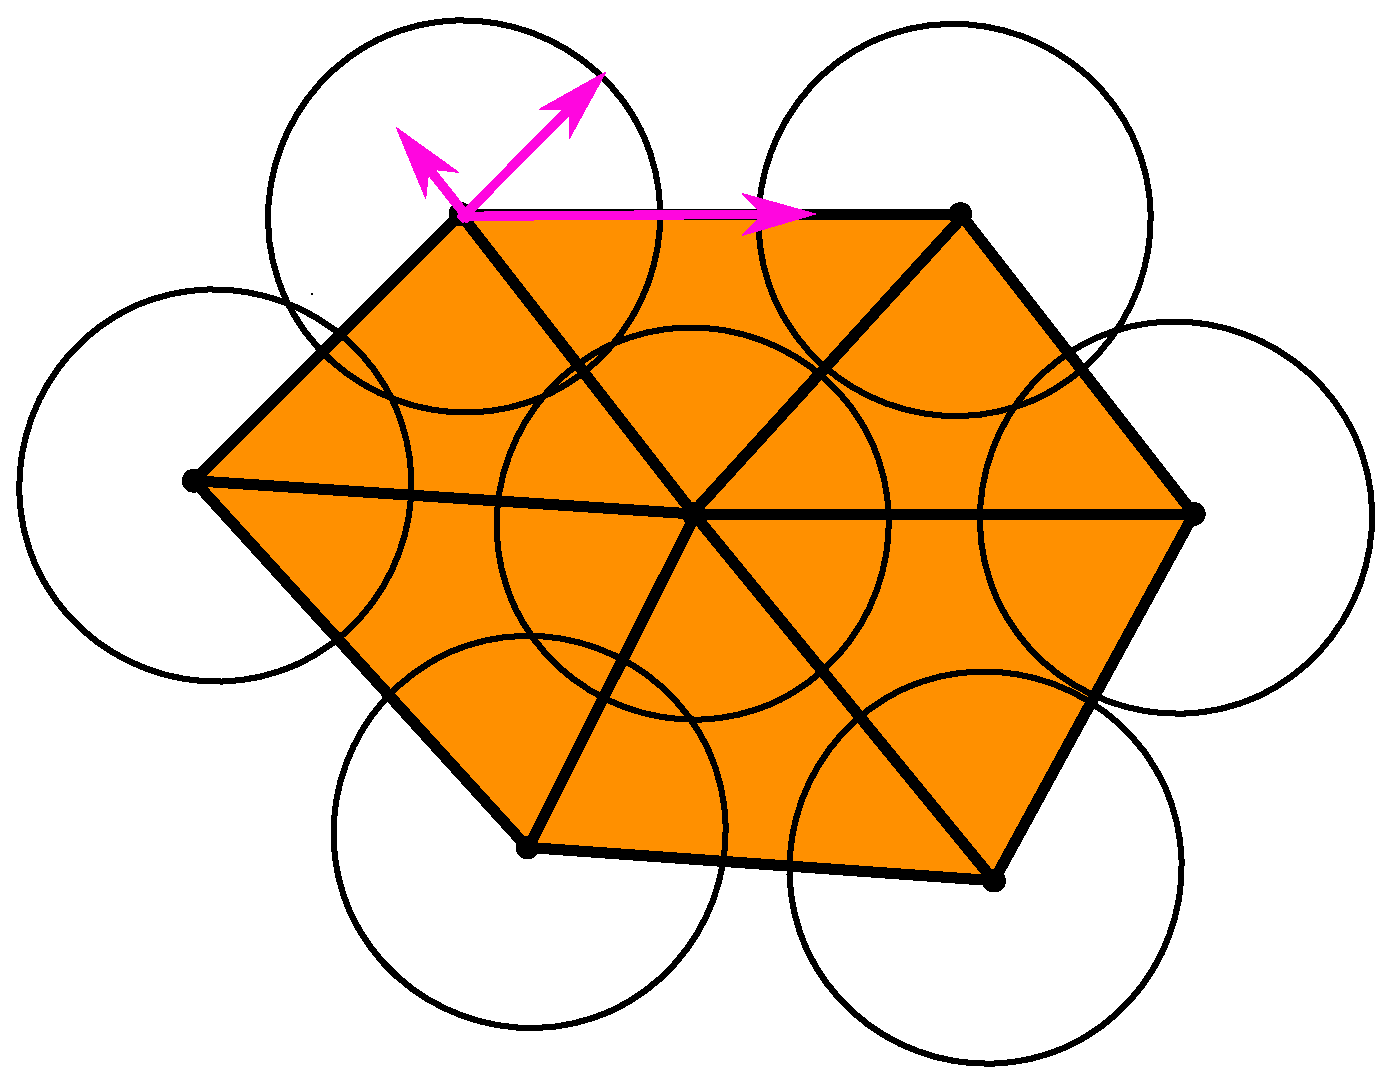
\includegraphics[width=\textwidth]{bilder/meshCorrector/EdgeLaw.eps}
      \caption[Kantenkräfte für optimale Kantenlängen]{Kantenkräfte für an einem Knoten \( k = 1 \). Die eingezeichneten Radien entsprechen \( \frac{l^{*}}{2} \).}
      \label{edgeLaw}
      \end{minipage}
      \hfill
      \begin{minipage}[t]{0.45\textwidth}
      \raisebox{10pt}{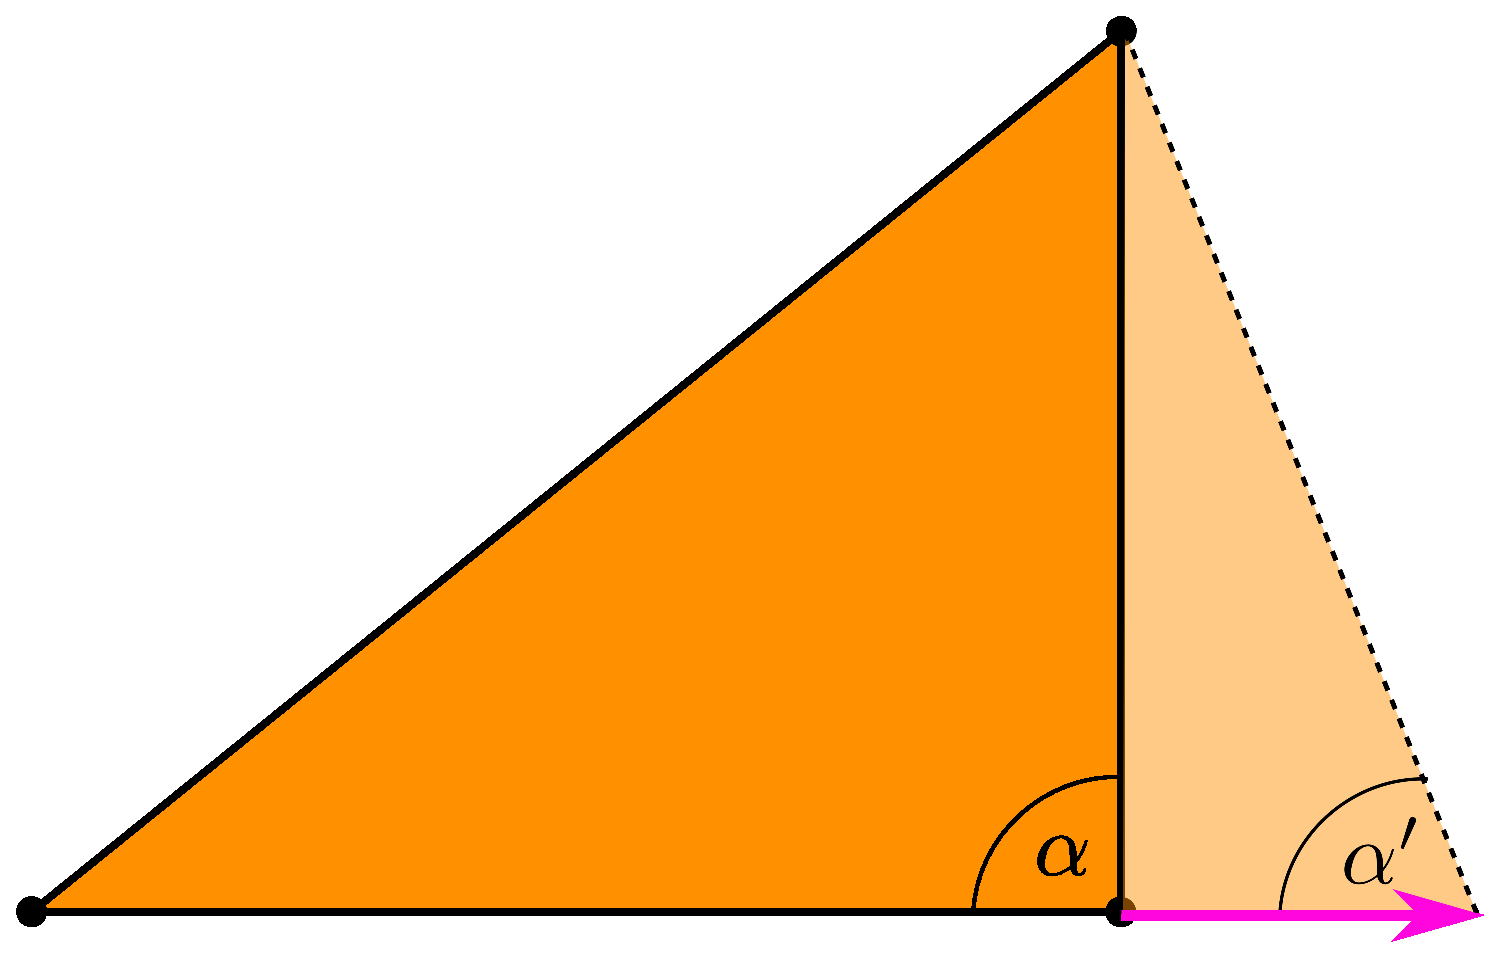
\includegraphics[width=\textwidth]{bilder/meshCorrector/AngleLaw.eps}}
      \caption[Winkeländerung durch Verschiebung]{Eine Verschiebung des Knotens entlang einer Kante verändert den Winkel.}
      \label{angleLaw}
      \end{minipage}
    \end{figure}

  \subsubsection{Optimale Winkel}
    Ein weiterer heuristischer Ansatz bezieht sich direkt auf die inneren Winkel eines Dreieckelements. 
    Wie in Abbildung \ref{angleLaw} angedeutet, bewirkt eine Verschiebung entlang der Kante eine Änderung des Winkels.
    Wird dabei, wie in Abbildung \ref{angleLaw}, die Kante länger, so wird der Winkel an dem zu verschiebenden Knoten kleiner, et vice versa. 
    Somit ist ein sinnvoller Ansatz für die Kraft an einem Knoten \( \sigma_{0} \) in Abhängigkeit 
    zur Kante \( \sigma^{1}_{i}\succ\sigma^{0} \) und dem Dreieck \( \sigma^{2}\succ\sigma^{1}_{i} \) 
    \begin{align}
       F^{A}_{\sigma^{0}\prec\sigma^{1}_{i}\prec\sigma^{2}} &:= \cos\measuredangle(\vec{e}_{0},\vec{e}_{1}) - c \label{angleForce}\\
                              &= \frac{\vec{e}_{0} \cdot \vec{e}_{1}}{\|\vec{e}_{0}\|\|\vec{e}_{1}\|} - c \\
       \vec{e}_{i} := \vec{e}_{\sigma^{1}_{i}} &= \vec{x}_{v_{i}} - \vec{x}_{\sigma^{0}}\\
    \end{align}
    mit \( i\in\{0,1\} \) und \( c\in[-1,1] \). 
    \( v_{i} \) ist also der Knoten, der mit \( \sigma^{0} \) die gemeinsame Kante \( \sigma^{1}_{i} \) 
    im Dreieck \( \sigma^{2} = [\sigma^{0},v_{0},v_{1}] \) hat.
    
    Eine sinnvolle Wahl für die Konstante ist \( c = \cos \frac{\pi}{3} = 0.5\).
    Sie würde in einer flachen Triangulation mit hexagonaler Struktur bewirken, dass sich keine Kräfte entwickeln, falls alle Dreiecke, bis auf Rotation und Translation, gleich sind.

  \subsubsection{Kombination der Kantenkräfte}
    Es hat sich gezeigt, dass \eqref{edgeForce} und \eqref{angleForce} gerade auf komplizierteren Gebieten einzeln entweder nicht das gewünschte Resultat liefern oder instabil sind.
    Deshalb kombinieren wir die beiden Kräfte linear:
    \begin{align}
      F^{\text{Gesamt}}_{\sigma^{0}\prec\sigma^{1}} &:= D \cdot F^{L}_{\sigma^{0}\prec\sigma^{1}} + (1-D) \cdot F^{A}_{\sigma^{0}\prec\sigma^{1}}
    \end{align}
    mit \( D\in[0,1] \).
    Algorithmus \ref{AlgoForces} zeigt, wie die resultierenden Kräfte auf einem Dreieckelement berechnet werden können. 
    Um alle Knotenkräfte\footnote{d.h. \((\vec{F}_{i})_{i=1,\ldots, N_{\sigma^{0}}}\in (\R^{3})^{N_{\sigma^{0}}} \)} zu erhalten, müssen wir nur noch die Element-Knotenkräfte aufassemblieren. 
    
  \subsubsection{Projektion der Kraftvektoren}
    Des Weiteren, wie im Algorithmus \ref{AlgoForces} zu sehen, wird der Kraftvektor \( \vec{F}_{i} \) in den Tangentialraum projiziert, das heißt
    \begin{align}
      \vec{F}_{T_{p}M,i} = \vec{F}_{i} - (\vec{F}_{i}\cdot\vec{\nu_{i}})\vec{\nu_{i}} \formkomma
    \end{align}
    wobei der Normalenvektor \( \vec{\nu_{i}}  \) am Knoten \( \sigma^{0}_{i} \) entweder als bekannt vorausgesetzt ist,
    über eine signierte Distanzfunktion \( \varphi \) ermittelt wird, also
    \begin{align}
      \vec{\nu_{i}} = \frac{\nabla\varphi}{\|\nabla\varphi\|}(\vec{x}_{i}) \formkomma
    \end{align}
    oder über die Elementnormalen approximiert wird
    \begin{align}
      \vec{\nu_{i}} = \sum_{\sigma^{2}\succ\sigma^{0}_{i}} \frac{|\sigma^{2}|}
                                                    {\sum_{\sigma^{2}\succ\sigma^{0}_{i}}|\sigma^{2}| } \vec{\nu}_{\sigma^{2}}
    \end{align}
    Somit kann im expliziten Eulerverfahren \eqref{euler} \( \vec{F}_{T_{p}M,i}\) statt \( \vec{F}_{i} \) verwendet werden.
    Das müssen wir nicht machen, aber es bringt Vorteile. 
    Zum einen könnten Knoten soweit in Normalenrichtung verschoben werden, dass die nachfolgende Projektion den Knoten falsch abbildet und das Gitter zerstört wird 
    (vgl. Abb. \ref{AbbFatalEuler}), zum anderen wird die Projektion in \eqref{euler} oft iterativ gelöst (vgl. \ref{SubSubSecPhiProject}) und je weiter weg wir den Knoten von der
    Mannigfaltigkeit verschieben, um so schlechter ist die Startnäherung für das iterative Verfahren.
    \begin{figure}
      \centering
      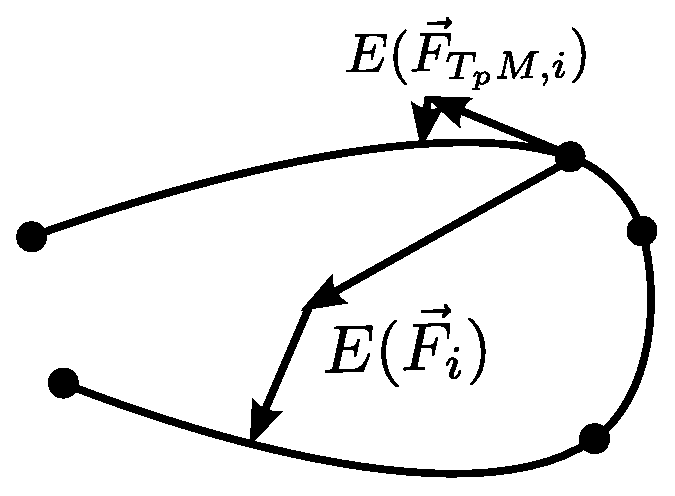
\includegraphics[width=0.5\textwidth]{bilder/meshCorrector/fatalEuler.eps}
      \caption[Euler mit und ohne Vorprojektion]{Eindimensionales Extrembeispiel für ein Schritt Euler-Explizit \( E \) (inkl. Nachprojektion \( \pi \))
                                                  eines Knotens mit und ohne Vorprojektion des Kraftvektors \( \vec{F}_{i} \)
                                                 zu \( \vec{F}_{T_{p}M,i}\). 
                                                 Ohne Vorprojektion kann es zu einem unzulässigen Gitter kommen.}
      \label{AbbFatalEuler}
    \end{figure}


  
  \subsection{Beispiele}
    
    \subsubsection{Ellipsoid}
      Wir wollen nun ein geeignetes Gitter für ein Ellipsoid erstellen (vgl. Appendix \ref{heineC}).
      Zur Verfügung steht uns eine Starttriangulierung der Einheitssphäre mit zirka 1000 Knoten.
      Es ist fast überall eine hexagonale Struktur vorhanden, bis auf 12 Defekte. 
      Genauer, an 12 Knoten
      befinden sich pentagonale 1-Ringe. 
      Dieses Startgitter wird nun auf den Ellipsoid projiziert (vgl. Abschnitt \ref{SubSubSecPhiProject}).
      
      Wie in Abbildung \ref{AbbEllipsoid} zu sehen, ist ein wohlzentrierter Simplizialkomplex nach nur
      wenigen Eulerschritten \eqref{euler} erreicht. 
      Der größte Winkel nimmt aber weiterhin logarithmisch ab. 
      Nach zirka 200 Schritten hat er sein Minimum erreicht und steigt danach wieder leicht an.
      Das ist nicht verwunderlich, denn kleinere Winkel sind nicht das einzige Optimalitätskriterium.
      Geplottet wurde das Integralmittel \( \bar{\alpha}_{\max} \) (\texttt{AvMaxAngle}) der größten Winkel der Dreiecke
      und der größte aller maximalen Winkel \(\alpha_{\max}^{\max} \) (\texttt{MaxMaxAngle}) nach jedem Iterationsschritt.
      \begin{align}
         \bar{\alpha}_{\max} &:= \frac{\int_{|K|}\alpha_{max}\mu}{\int_{|K|}\mu}
                              = \frac{1}{V(K)} \sum_{\sigma^{2}\in K} |\sigma^{2}| \alpha_{max}^{\sigma^{2}} \\
         \alpha_{\max}^{\max} &:= \max\left\{ \alpha_{max}^{\sigma^{2}} \middle| \sigma^{2} \in K \right\}
      \end{align}
      Wobei \( |K| \) der zugrunde liegende Raum des Simplizialkomplexes \( K \) 
      und \( \mu\in\Lambda^{2}(|K|) \) die stückweise konstante Volumenform auf \( |K| \) ist.
      \( \alpha_{max}^{\sigma^{2}} \) ist der größte Winkel auf dem Dreieck \( \sigma^{2} \).

      \begin{figure}
        \begin{minipage}[t]{0.45\textwidth}
        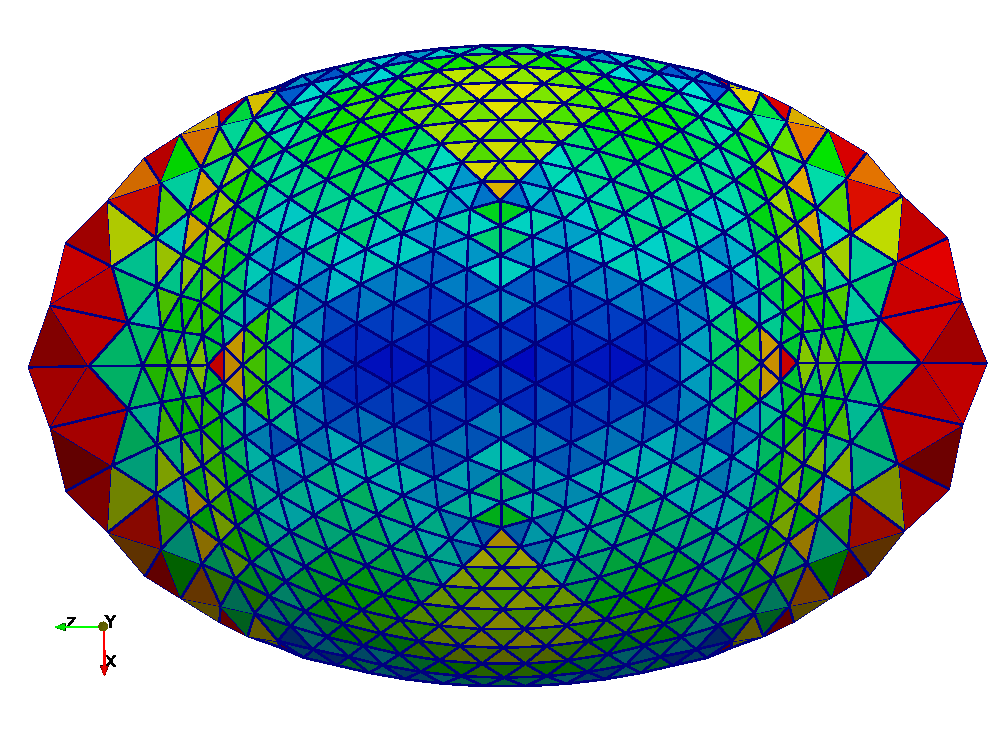
\includegraphics[width=\textwidth]{bilder/meshCorrector/Before_AnglesHeine51c_1k_h001_k10_c07.eps}
        \end{minipage}
        \hfill
        \begin{minipage}[t]{0.49\textwidth}
        \includegraphics[width=\textwidth]{bilder/meshCorrector/step7_AnglesHeine51c_1k_h001_k10_c07.eps}
        \end{minipage}
        \begin{minipage}[t]{0.49\textwidth}
        \includegraphics[width=\textwidth]{bilder/meshCorrector/step1000_AnglesHeine51c_1k_h001_k10_c07.eps}
        \end{minipage}
        \hfill
        \begin{minipage}[t]{0.5\textwidth}
        \includegraphics[width=\textwidth]{bilder/meshCorrector/step7500_AnglesHeine51c_1k_h001_k10_c07.eps}
        \end{minipage}
        \begin{minipage}[t]{\textwidth}
        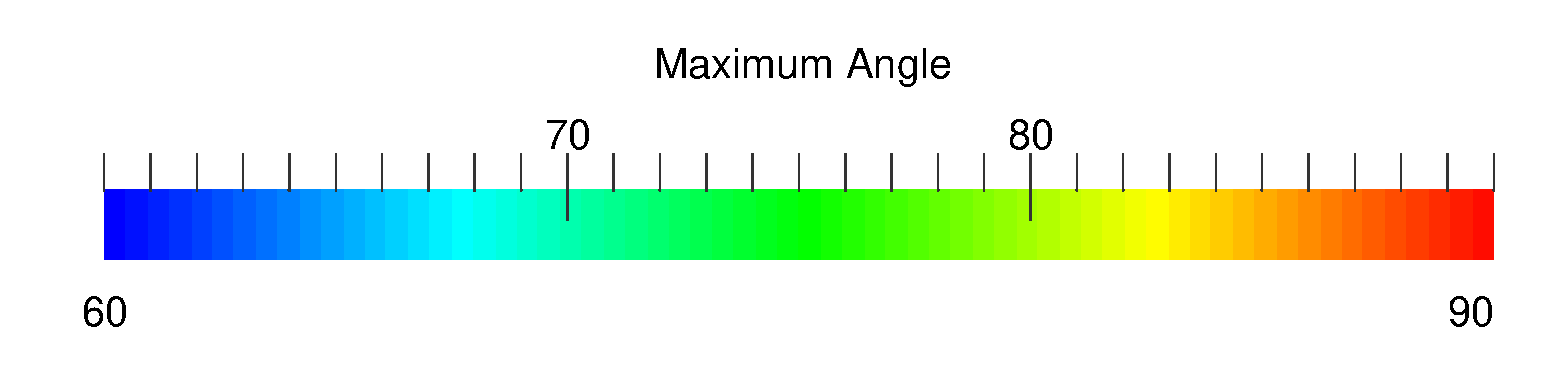
\includegraphics[width=\textwidth]{bilder/meshCorrector/Angle6090_scaleBar.eps}
        \end{minipage}
        \caption[Gittergenerierung: Ellipsoid]
                {Parameter: h = 0.01; k = 1; c = 0.7. 
                 Von links oben nach rechts unten: 
                 Startgitter (keine Wohlzentriertheit, maximaler Winkel ca. \ang{95.9}); 
                 nach 7 Eulerschritten (Wohlzentriertheit);
                 nach 1000 Eulerschritten (danach keine signifikanten Veränderungen mehr);
                 (semilog)Eulerschritte-Winkel-Plot (Maximum und Integralmittel)}
         \label{AbbEllipsoid}
        \begin{minipage}[t]{0.32\textwidth}
        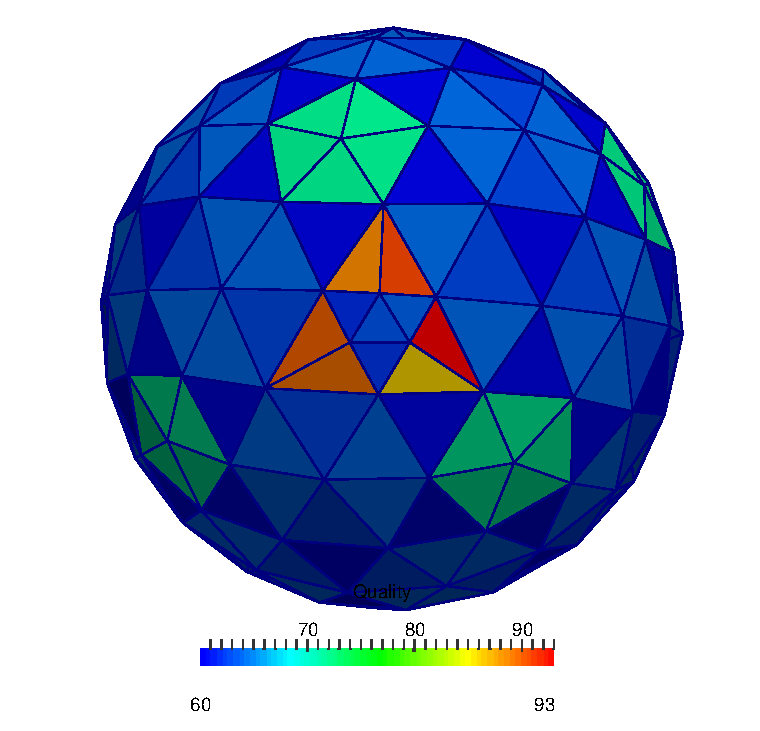
\includegraphics[width=\textwidth]{bilder/meshCorrector/sphereDivBy4Before.eps}
        \end{minipage}
        \hfill
        \begin{minipage}[t]{0.32\textwidth}
        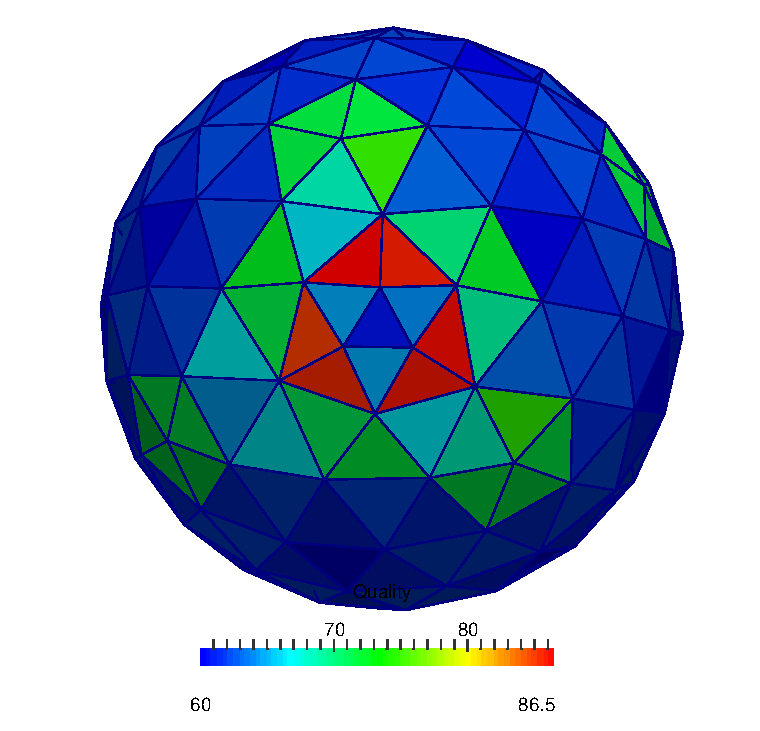
\includegraphics[width=\textwidth]{bilder/meshCorrector/sphereDivBy4AfterH01K1C07_1Step.eps}
        \end{minipage}
        \begin{minipage}[t]{0.32\textwidth}
        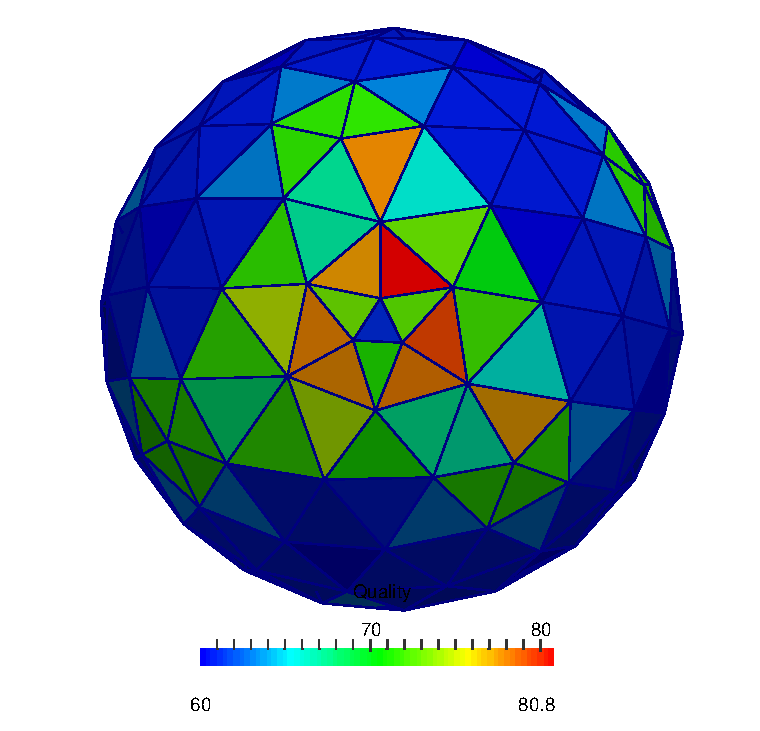
\includegraphics[width=\textwidth]{bilder/meshCorrector/sphereDivBy4AfterH008K03C07_1Step.eps}
        \end{minipage}
        \hfill
        \caption[Gittergenerierung: Lokale Verfeinerung]
                 {Von links nach rechts: 
                 Startgitter; 
                 nach 1 Eulerschritt (h = 0.1, k = 1, c = 0.7, max. Winkel ca. \ang{86.5});
                 nach 1 Eulerschritt (h = 0.08, k = 0.3, c = 0.7, max. Winkel ca. \ang{80.8})}
         \label{AbbVerfeinerung}
      \end{figure}

    \subsubsection{Lokale Verfeinerung}
     
      %\begin{figure}
      %\end{figure}

      Die in der FEM häufig anzutreffende Verfeinerung, nämlich die Halbierung der Dreiecke, führt zu 1-Ringen aus 4 Flächenelementen an den neu
      entstandenen Knoten und ist somit im Allgemeinen nicht zulässig für unsere Triangulierung.
      Eine Möglichkeit Dreiecke zu verfeinern und trotzdem eine Ausgangssituation für ein wohlzentriertes Gitter zu schaffen, ist das Vierteln von
      Flächenelementen, wobei 3 neue Knoten an den Seitenhalbierenden enstehen (siehe Abb. \ref{AbbVerfeinerung} ganz links). 
      Die somit hängenden Knoten werden beseitigt, indem die Nachbarelemente halbiert werden.
      Das heißt es ensteht hexagonale Struktur an einem neuen Knoten, wenn beide angrenzenden Dreiecke zum Verfeinern markiert wurden und
      pentagonale Struktur, wenn nur ein Dreieck markiert wurde. 
      Für die alten Knoten an denen eine neue Kante hinzu kommt, erhöht sich die Anzahl
      der umliegenden Flächenelemente um eins.

      Nachdem die neuen Knoten auf die Mannigfaltigkeit projiziert werden, ist im Allgemeinen noch nicht sichergestellt, dass eine wohlzentrierte
      Triangulation vorliegt. Deshalb wenden wir unseren Algorithmus \eqref{euler} darauf an.
      Wenn vor der Verfeinerung ein zulässiges Gitter vorlag, dann zeigt sich, dass wir nur sehr wenige Iterationsschritte benötigen, um
      wieder ein
      zulässiges Gitter herzustellen. Abbildung \ref{AbbVerfeinerung} zeigt das Resultat nach nur einem Eulerschritt mit zwei verschiedenen
      Parameterkonfigurationen. Hier wurde ein Dreieck verfeinert (links). Das Gitterverbesserungsverfahren erzeugt zum einen wohlzentrierte
      Dreiecke bei denen die Abmessungen weitestgehend gleich bleiben (Mitte) und bei denen die neu entstandenen Elemente schrumpfen,
      jedoch die Winkel
      besser sind (rechts), als bei der anderen Parameterkonfiguration.

     \begin{fazit}
        Prinzipiell ist es also möglich ein wohlzentriertes Gitter aus einer Ausgangstriangulation zu erzeugen, wenn genügend viele
        Informationen über die stetige Oberfläche bekannt sind. 
        Zum Teil reichen auch nur wenige Eulerschritte aus, um Wohlzentriertheit zu erreichen, jedoch um in gewissem Sinne gleichmäßige
        Gitter zu bekommen, muss wesentlich mehr Aufwand betrieben werden, der unter Umständen den des eigentlichen Problems, wie das Lösen
        einer Partiellen Differentialgleichung auf der Oberfläche, bei weitem übersteigt.
     \end{fazit}




  \newpage
  \section{Implizit gegebene Oberflächen}
    \label{secImpliziteMannigfaltigkeiten}
    Oftmals ist eine Oberfläche \( M\subset\R^{3} \) nicht explizit über eine Parametrisierung 
    \begin{align}
      X:(u,v)\mapsto X(u,v)\in\R^{3}
    \end{align}
    gegeben, sondern über den 0-Level-Set einer signierten Distanzfunktion \( \varphi:\R^{3}\rightarrow\R \).
    Die 2-Mannigfaltigkeit kann dann durch 
    \begin{align}
      M = \left\{ \vec{x}\in\R^{3} \middle| \varphi(\vec{x})=0 \right\} \text{.}
    \end{align}
    beschrieben werden.
    Solche implizit beschriebenen Oberflächen liegen zum Beispiel bei dreidimensionalen Phasenfeldproblemen vor 
    (z.B. Allen-Cahn-, Cahn-Hilliard- oder Phase-Field-Crystal-Modell). 
    Die Distanzfunktion\footnote{auch Phasen- oder Ordnungsfunktion genannt} \( \varphi\) ist dort gerade die Lösung dieser Probleme
    und das Null-Niveau dieser Funktion beschreibt die Phasengrenzen.

    Wir treffen hier die Konvention, dass "`außen"' \( \varphi > 0 \) gilt und "`innen"' \( \varphi < 0 \).
    Dadurch zeigt der Gradient \( \nabla\varphi(\vec{x}) \) für alle \( \vec{x}\in M \) in Richtung der äußeren Normalen.
    "`Außen"' und "`innen"' ist durch die Orientierung der Mannigfaltigkeit gegeben. 
    In Falle von 2"~Mannigfaltigkeiten ohne Rand, ist "`innen"' gerade das von der Oberfläche umschlossene Gebiet im \( \R^{3} \).

    \subsection{Numerische Projektion}
      \label{SubSubSecPhiProject}
      Wenn bei einem Simplizialkomplex, welches die Oberfläche approximiert, neue Knoten entstehen oder vorhandene verschoben werden sollen,
      dann ist es notwendig diese Knoten auf die Mannigfaltigkeit zu projizieren, 
      denn eine Bedingung an den Simplizialkomplex ist, dass die Knoten dort und auf dem abstrakten Simplizialkomplex übereinstimmen.

      Gesucht ist also das
      \begin{align}
        \argmin_{\vec{x}\in M} \|\vec{y} - \vec{x}\|
      \end{align}
      für den Knoten mit den Koordinaten \( \vec{y}\in\R^{3}\setminus M \), der sich noch nicht auf der Mannigfaltigkeit \( M \) befindet 
      und damit \( \varphi(\vec{y}) \neq 0 \) gilt.

      \begin{figure}
        \centering
        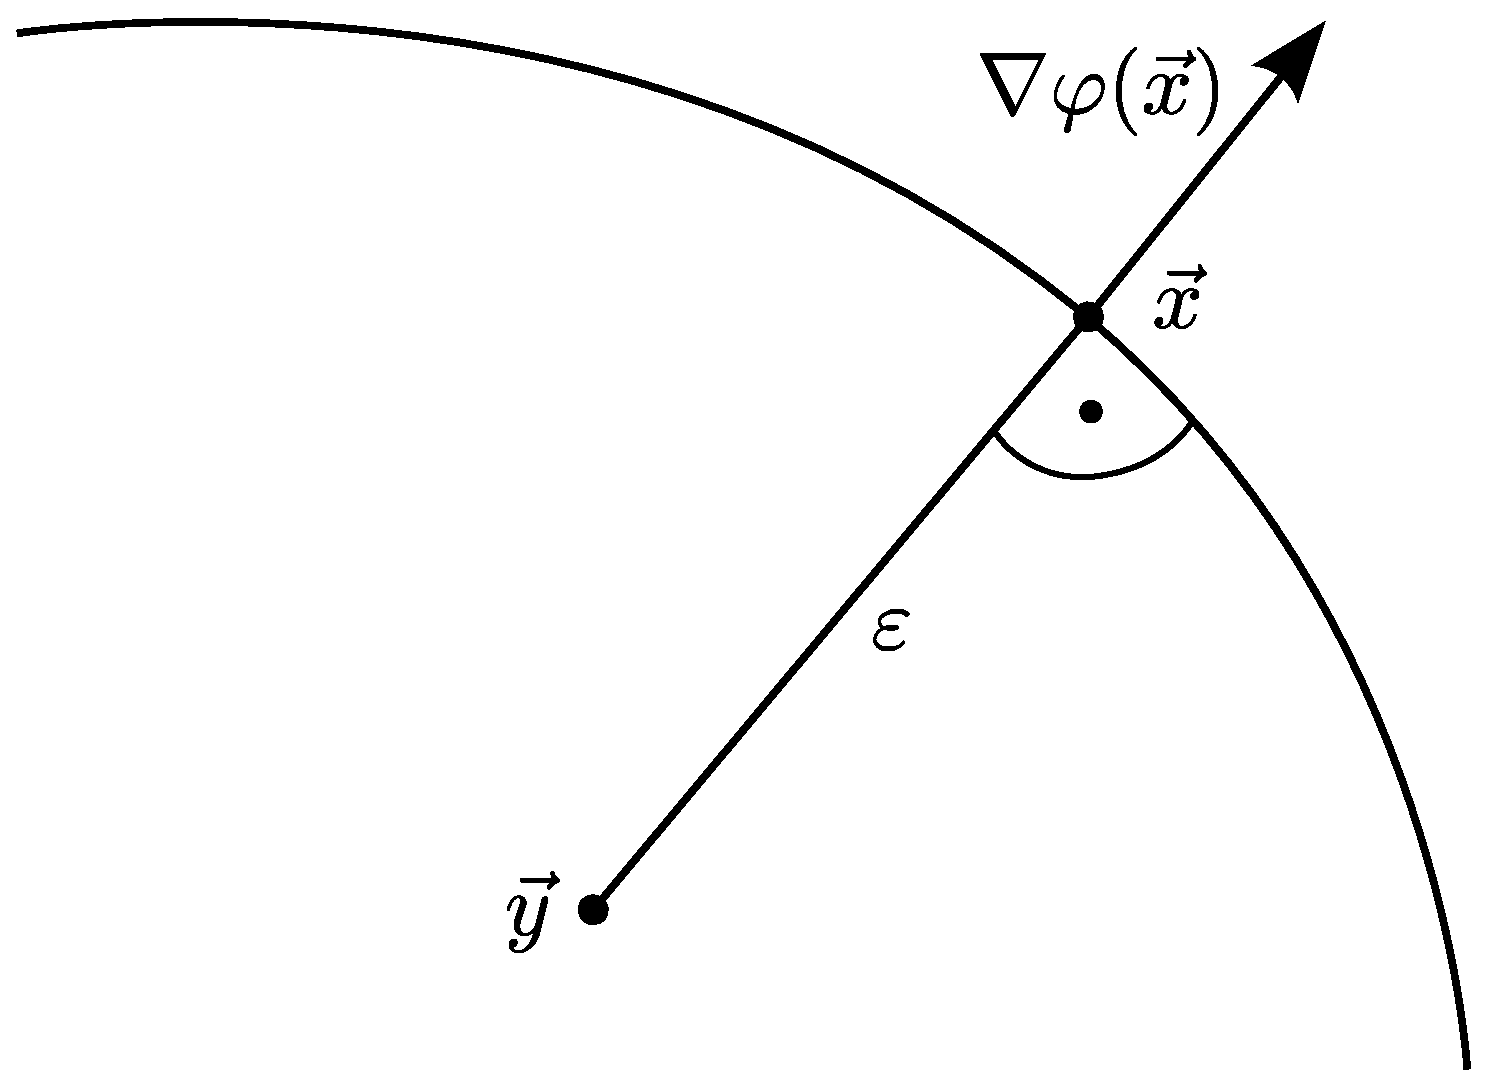
\includegraphics[width=0.5\textwidth]{bilder/projection/projection.eps}
        \caption[Projektion]{Darstellung des Punktes \( \vec{y} \) und dessen projizierter Punkt \( \vec{x} \)}
        \label{AbbProjection}
      \end{figure}
      Der kürzeste Weg mit Länge \( \varepsilon \) steht im rechten Winkel zur Oberfläche am Punkt \( \vec{x} \) (siehe Abb. \ref{AbbProjection}).
      Für den gesuchten Punkt \( \vec{x}\in M \subset \R^{3} \) folgt somit
      \begin{align}
        \vec{x} &= \vec{y} + \frac{\varepsilon}{\|\nabla\varphi(\vec{x})\|} \nabla\varphi(\vec{x})
                = \vec{y} + h \nabla\varphi(\vec{x}) \label{EqProjection}
      \end{align}
      für \( \varepsilon = h \|\nabla\varphi(\vec{x})\| \).
      Allerdings ist weder \( h \) noch \( \vec{x} \) bekannt. 
      Deshalb approximieren wir den Gradienten mittels Taylor an \( \vec{y} \):
      \begin{align}
        \nabla\varphi(\vec{x}) &= \nabla\varphi(\vec{y}) + H[\varphi](\vec{y})(\vec{x}-\vec{y}) + HOT \\
                               &= \nabla\varphi(\vec{y}) + \frac{\varepsilon}{\|\nabla\varphi(\vec{x})\|} H[\varphi](\vec{y})\nabla\varphi(\vec{x}) + HOT \formkomma
      \end{align}
      wobei  \( HOT \) für Therme höherer Ordnung (in \( \varepsilon \)) steht 
      und \( H[\varphi] \) die (symmetrische) Hessematrix von \( \varphi \in
      C^{2}\left(\overline{B_{\varepsilon}(\vec{x})}\right) \) ist.
      Einsetzen in \eqref{EqProjection} liefert
      \begin{align}
        \vec{x} &= \vec{y} +  h \nabla\varphi(\vec{y}) + \vec{O}(\varepsilon^{2}) \quad\text{.}
      \end{align}
      Somit ist für uns die Abschätzung 
      \begin{align}
        \vec{x}^{*} &:= \vec{y} +  h \nabla\varphi(\vec{y})
      \end{align}
      für \( \vec{x} \) ausreichend, falls \( \varphi \) hinreichend glatt und \( \varepsilon \) klein.

      Nun wollen wir \( h \) so bestimmen, dass \(\vec{x}^{*}\) auf der Oberfläche liegt, das heißt
      \begin{align}
        \Phi_{\vec{y}}(h) := \varphi(\vec{x}^{*}) = \varphi(\vec{y} +  h \nabla\varphi(\vec{y})) = 0 \quad\text{.}
      \end{align}
      Dieses Nullstellenproblem lösen wir in erster Näherung mittels Newton-Verfahren und Startlösung \( h=0 \).
      \begin{align}
        \hat{h} &= - \frac{\Phi_{\vec{y}}(0)}{\Phi'_{\vec{y}}(0)}
                = - \frac{\varphi(\vec{y})}{\|\nabla\varphi(\vec{y})\|^{2}}
      \end{align}
      Damit stellen wir die Iterationsvorschrift
      \begin{align}
        \vec{y}_{i+1} &:= \vec{y}_{i} - \frac{\varphi(\vec{y}_{i})}{\|\nabla\varphi(\vec{y}_{i})\|^{2}}  \nabla\varphi(\vec{y}_{i})
                       %% \overset{i\rightarrow\infty}{\longrightarrow}  \vec{x}^{*}
      \end{align}
      auf.
      Diese numerische Projektion, die wir hier nun erhalten haben, ist für unsere Zwecke vollkommen ausreichend und lieferte in allen
      Berechnungen, die im Rahmen dieser Arbeit gemacht wurden, ausgezeichnete Ergebnisse.
      Als Abbruchskriterium wurde fast immer \( \varphi(\vec{y}) < 1.0E-8 \) gewählt, das nach wenigen Iterationsschritten erreicht wurde.


